\documentclass[conference]{IEEEtran}
\IEEEoverridecommandlockouts
% The preceding line is only needed to identify funding in the first footnote. If that is unneeded, please comment it out.
%Template version as of 6/27/2024

\usepackage{cite}
\usepackage{amsmath,amssymb,amsfonts}
\usepackage{algorithmic}
\usepackage{graphicx}
\usepackage{textcomp}
\usepackage{xcolor}
\usepackage{subcaption}
\usepackage{booktabs}
\usepackage{url}
\usepackage{microtype}
\usepackage{listings}

\def\BibTeX{{\rm B\kern-.05em{\sc i\kern-.025em b}\kern-.08em
		T\kern-.1667em\lower.7ex\hbox{E}\kern-.125emX}}

% Listings configuration
\lstset{
	basicstyle=\ttfamily\footnotesize,
	breaklines=true,
	breakatwhitespace=true,
	frame=single,
	columns=fullflexible,
	keepspaces=true
}

\begin{document}
	
	\title{The EC2 Sweet Spot: A Cost-Efficiency Analysis of Video Codecs on AWS T-Family Instances}
	
	\author{
		\IEEEauthorblockN{bjrv,cagf}
		\IEEEauthorblockA{esses detalheszinhos ainda vou ajeitar, o mais importante é o conteúdo}
	}
	
	\maketitle
	
	\begin{abstract}
		The diverse landscape of cloud instance types presents optimization challenges for video compression workloads. This study analyzes cost-efficiency of burstable compute instances for video encoding tasks. Benchmarking shows that while instances with 8 vCPUs demonstrated 40.5\% faster compression times than instances with 2 vCPUs, smaller configurations proved 20× more cost-efficient. This finding motivated a two-phase case study comparing horizontally-scaled clusters against vertically-scaled instances. By eliminating a provisioning bottleneck using custom machine images, an optimized ten-instance cluster achieved total processing time of 1.45 minutes, representing 1.28× speedup over the 1.85 minutes required by a single powerful instance with 75.5\% cost reduction. For divisible workloads, parallel architectures utilizing cost-optimized instances provide improved strategies for balancing performance and economic efficiency in cloud environments.
	\end{abstract}
	
	\begin{IEEEkeywords}
		AWS EC2, FFmpeg, Docker, Video Codecs, Cloud Performance, Cost Optimization, Parallel Encoding, Benchmarking
	\end{IEEEkeywords}
	
	\section{Introduction}
	
	Cloud computing has transformed how businesses deploy computing resources, with Cloud Service Providers offering diverse instance types that present significant cost-performance optimization challenges for video compression workloads \cite{b1,b17}. This study focuses on AWS T-family instances, low-cost options with CPU bursting capability that enable a disposable worker pattern for short, intensive tasks like video segment compression. Our research quantifies this strategy's cost-effectiveness, identifying where T-family economies outweigh fixed-performance alternatives.
	
	While cloud optimization has advanced, media processing cost-efficiency requires further investigation, particularly regarding scaling trade-offs and operational overhead. Our contributions include: systematic evidence challenging larger instance superiority, showing smaller burstable instances achieve up to \textbf{20× higher cost-efficiency}; quantification of \textbf{70\% provisioning overhead} in parallel encoding; an AMI optimization framework reducing time and costs by \textbf{55.9\%}; and empirical demonstration that optimized horizontal scaling delivers \textbf{1.28× faster} processing with \textbf{75.5\% cost reduction}.
	
	We characterize burstable instance performance for video compression to enable cost-effective selection. Our methodology addresses three objectives: comparing T-family instance performance (t2.micro to t3.2xlarge); evaluating codec impact (H.264, H.265, VP9); and proposing resource allocation guidelines. Building on \cite{b3}, we confirm hardware heterogeneity across availability zones (detailed in Section \ref{met:validation-processor-homogeneity}) and conduct extensive compression tests to provide performance insights.
	
	Section~\ref{rel_works} reviews cloud optimization and video processing literature. Section~\ref{met} details our methodology across three phases. Section~\ref{experiments} presents corresponding results, and Section~\ref{conclusion} summarizes contributions and future directions.
	
	\section{Related Works}
	\label{rel_works}
	
	Video processing computational resource optimization presents research challenges due to modern codec complexity. Advanced standards like Versatile Video Coding (VVC) introduce sophisticated tools that increase computational demands, driving research into algorithmic optimizations \cite{b15, b16}. While prior work, such as that by \textbf{Dancheva et al.} \cite{b3}, focuses on comparative encoding performance, our investigation shifts the focus to the cloud infrastructure itself, analyzing its performance and cost-effectiveness for practical deployment.
	
	Cloud resource optimization has been studied from multiple perspectives. Prior work includes cost-driven provisioning methodologies for scientific computing, as demonstrated by \textbf{Álvarez et al.} \cite{b2}, and surveys categorizing resource management strategies \cite{b4}. Our research extends this foundation by demonstrating that properly optimized horizontal architectures can simultaneously outperform vertical scaling for video encoding workloads in both processing speed and cost-efficiency.
	
	Recent work by \textbf{Jiang et al.} \cite{b20} introduces PIVOT, a cloud-agnostic framework that addresses cost-aware scheduling in multi-cloud environments. Their approach tackles significant challenges in cross-cloud data analysis, including infrastructure heterogeneity and prohibitive egress costs. While PIVOT focuses on multi-cloud workflow orchestration for big data applications, our work complements this by providing a granular analysis of cost-performance trade-offs within a single cloud provider's burstable instance family, specifically for video encoding workloads.
	
	The multi-objective nature of cloud optimization problems has been well-established. Studies such as \textbf{Katsenou et al.} \cite{b8} provide thorough analyses of energy efficiency trade-offs across different codecs and hardware platforms. Conversely, recent comprehensive analyses like \textbf{Maas et al.} \cite{b1} offer detailed investigations of cost-performance balances across a wide range of cloud instances. Our work aligns with this latter approach but introduces a specialized focus on burstable instance families and parallel encoding architectures, with particular emphasis on quantifying operational overheads.
	
	Benchmarking methodologies represent a critical dimension of cloud performance research. Broad comparative studies illustrate the heterogeneity in cloud technologies, highlighting challenges in establishing direct performance comparisons \cite{b18, b1}. Our methodology addresses this challenge through environmental standardization, using containerized execution environments that align with the reproducible frameworks advocated by studies such as \textbf{Ferreira et al.} \cite{b9}.
	
	Our research addresses cloud performance variability through empirical measurement. We quantify variability across 30 trials per configuration, establishing baseline performance profiles for cost-efficiency analysis. This data-driven approach complements predictive modeling techniques proposed in prior work \cite{b10, b11}.
	
	The architectural principles underlying our parallel processing case study draw from established distributed systems concepts. The fundamental strategy of decomposing large, divisible workloads to optimize cost efficiency has been demonstrated in contexts such as task scheduling in fog-cloud environments \cite{b12, b13}. Our contribution lies in applying these principles to a specialized yet practically significant domain: parallel video encoding within public cloud infrastructure, with particular emphasis on quantifying and mitigating provisioning overhead.
	
	\begin{table*}[!htbp]
		\centering
		\caption{Systematic comparison of related works in cloud resource optimization and video processing}
		\label{tab:comparative_analysis}
		\begin{tabular}{|p{0.15\linewidth}|p{0.18\linewidth}|p{0.28\linewidth}|p{0.28\linewidth}|}
			\hline
			\textbf{Study} & \textbf{Focus} & \textbf{Contributions} & \textbf{Gaps Addressed} \\
			\hline
			Álvarez et al. \cite{b2} & Scientific workloads & Cost-aware provisioning & No media processing focus \\
			\hline
			Dancheva et al. \cite{b3} & Video encoding performance & Encoding time comparison & Limited cost analysis \\
			\hline
			Jiang et al. \cite{b20} & Multi-cloud scheduling & Cost-aware framework for cross-cloud workflows & Big data focus, limited video processing analysis \\
			\hline
			Maas et al. \cite{b1} & Broad cloud benchmarking & Instance performance analysis & No video encoding specialization \\
			\hline
			Ferreira et al. \cite{b9} & Benchmarking methodologies & Reproducible frameworks & No video encoding application \\
			\hline
			Katsenou et al. \cite{b8} & Energy efficiency & Codec energy analysis & Embedded devices focus \\
			\hline
			\textbf{Our Work} & \textbf{Burstable instances for video encoding} & 
			\scriptsize
			\begin{itemize}
				\vspace{-0.2cm}
				\item Size-efficiency trade-offs
				\item Overhead quantification  
				\item AMI optimization
				\item Scaling comparison
				\vspace{-0.2cm}
			\end{itemize}
			& 
			\scriptsize
			\begin{itemize}
				\vspace{-0.2cm}
				\item Burstable instance focus
				\item Parallel overhead measurement
				\item Divisible workload optimization
				\item Practical AMI strategies
				\vspace{-0.2cm}
			\end{itemize}
			\\
			\hline
		\end{tabular}
	\end{table*}
	
	Table~\ref{tab:comparative_analysis} provides a systematic comparison of related research, illustrating how our work complements and extends existing literature. While previous studies have established valuable foundations in their respective domains, our research provides an integrated analysis specifically addressing cost-efficiency trade-offs in burstable instances and parallel video encoding architectures, with particular emphasis on operational overhead quantification and practical optimization strategies that bridge identified research gaps.
	
	\section{Experimental Methodology}
	\label{met}
	
	This research employed a systematic experimental methodology to investigate the relationship between computational cost and performance for video encoding tasks in cloud environments. The study was conducted utilizing AWS infrastructure in the us-east-1 region. Our methodological approach comprised three principal phases conducted sequentially:
	
	\subsection{Phase 1: Validation of Processor Homogeneity}
	\label{met:validation-processor-homogeneity}
	
	To ensure experimental validity and mitigate potential confounding factors from hardware heterogeneity, we implemented a comprehensive verification protocol for hardware configuration consistency across computational instances.
	
	\subsubsection{Instance Provisioning Protocol}
	We deployed \textbf{100 instances of each configuration type} spanning the burstable instance spectrum (t2.micro, t3.micro, t3.small, t3.medium, t3.large, t3.xlarge, and t3.2xlarge) across all availability zones (a through f) within the us-east-1 region. All instances were initialized with \textbf{Ubuntu 22.04 LTS} to maintain environmental consistency.
	
	\subsubsection{Computational Specification Verification}
	Each provisioned instance executed the \texttt{cat /proc/cpuinfo} command to extract detailed processor specifications including architectural model, clock frequency, cache hierarchy, and virtual core allocation. The collected hardware metadata was transmitted to a centralized analysis server for aggregation and comparative assessment.
	
	\subsubsection{Heterogeneity Characterization}
	\label{met:heterogeneity-detection-item}
	Our analysis confirmed hardware variation across availability zones, consistent with prior cloud infrastructure studies \cite{b2, b5, b6, b7}. For minimal instances in zone \texttt{a}, processors were distributed between \textbf{Intel(R) Xeon(R) Platinum 8175M} and \textbf{8259CL} microarchitectures, with the latter predominant (Table \ref{tab:processors}).
	
	\begin{table}[htbp]
		\centering
		\caption{Computational heterogeneity characterization in minimal instances within us-east-1 region, illustrating processor model distribution across availability zones}
		\label{tab:processors}
		\begin{tabular}{|c|c|c|}
			\hline
			Availability Zone & Processor Architecture & Instance Count \\ \hline
			a & Xeon(R) 8175M @ 2.50GHz & 2 \\ \hline
			a & Xeon(R) 8259CL @ 2.50GHz & 98 \\ \hline
			f & Xeon(R) 8175M @ 2.50GHz & 26 \\ \hline
			f & Xeon(R) 8259CL @ 2.50GHz & 74 \\ \hline
		\end{tabular}
	\end{table}
	
	\subsubsection{Experimental Control Strategy}
	To mitigate processor heterogeneity effects, we selected \textbf{availability zone `a`} and used the \textbf{statistically dominant CPU architecture} for each instance type. Each VM underwent architectural validation, with non-conforming instances discarded and replaced. Benchmarking proceeded only when processor specifications matched predefined requirements.
	
	This systematic methodological approach ensured all subsequent experiments were conducted under controlled computational conditions, thereby preserving the internal validity of performance comparisons.
	
	\subsection{Phase 2: Initial Performance Benchmarks}
	\label{execution-initial-performance-benchmarks}
	
	\subsubsection{Experimental Environment Configuration}
	
	Following computational homogeneity validation, we established dedicated experimental instances for video compression evaluation, with one instance per configuration type allocated for each encoding algorithm.
	
	\textbf{Containerized Execution Environment}
	
	To ensure experimental reproducibility and environmental consistency, we employed a customized Docker container architecture. This approach \textbf{eliminated the need for} traditional on-instance software compilation, accelerating deployment cycles while enhancing methodological reproducibility. The container environment was pre-configured with a production-ready FFmpeg implementation and codec support.
	
	The containerized execution model guaranteed identical software stacks across all experimental instances, eliminating potential confounding variables related to library versions, compilation flags, or system dependencies. The integrated FFmpeg build provided complete support for the investigated video compression standards:
	\begin{itemize}
		\item \textbf{H.264/AVC (Advanced Video Coding)}
		\item \textbf{H.265/HEVC (High Efficiency Video Coding)}
		\item \textbf{VP9 (WebM Project)}
	\end{itemize}
	
	Prior to benchmark initiation, we conducted container integrity verification and functional validation of FFmpeg and all codec implementations on designated test instances.
	
	\textbf{Experimental Workload Specification}
	The video content utilized for experimental evaluation was sourced from the public repository \textbf{sample-videos.com} and temporally segmented to a standardized 30-second duration. This methodological decision ensured that experiments completed within operationally feasible timeframes while avoiding pathological execution durations that could compromise statistical significance.
	
	\subsubsection{Experimental Execution Protocol}
	
	Each experimental condition was replicated \textbf{30 times} to establish statistical robustness and account for performance variability inherent in cloud environments. The experimental design incorporated varying degrees of parallelization to evaluate performance scaling characteristics.
	
	Video Encoding Experimental Procedure
	Video compression performance was evaluated using the three designated encoding algorithms (H.264, H.265, VP9). The following standardized \textbf{FFmpeg} command template was executed within the containerized environment for each encoding task:
	\begin{center}
		{\ttfamily\scriptsize
			\fbox{
				\begin{minipage}{0.9\linewidth}
					ffmpeg -i input.mp4 -c:v <codec> -preset slow -b:v 2M \\
					\hspace{15pt}-threads <n> output.mp4
				\end{minipage}
			}
		}
	\end{center}
	
	Where:
	\begin{itemize}
		\item The \texttt{<codec>} parameter evaluated three compression standards: \texttt{libx264}, \texttt{libx265}, and \texttt{libvpx-vp9}.
		\item The \texttt{<n>} parameter was experimentally manipulated across values of 1, 3, 5, and 10 threads. This range was strategically selected to evaluate performance scalability across diverse scenarios: single-threaded execution, parallelization approximating typical virtual core counts of smaller instances, and extended thread configurations to assess hyper-threading efficiency and scheduling overhead on larger instances.
		\item The \textbf{total encoding duration} was precisely recorded, and the \textbf{computational cost per encoding operation} was calculated based on the published hourly pricing for each instance configuration.
	\end{itemize}
	
	\subsection{Phase 3: Horizontal vs. Vertical Scaling Analysis}
	
	Building upon the foundational performance benchmarks, we designed a structured two-phase case study to comparatively analyze the operational efficiency of horizontal versus vertical scaling strategies for substantial video encoding workloads.
	
	\subsubsection{Experimental Workload and Architectural Configurations}
	\begin{itemize}
		\item \textbf{Experimental Workload:} A single 10-minute high-resolution video file served as the standardized workload for all case study experiments.
		\item \textbf{Architectural Configurations:}
		\begin{itemize}
			\item \textbf{Horizontal Scaling (Scale-Out Architecture):} The 10-minute video was partitioned into 10 temporally contiguous one-minute segments. Ten minimal computational instances (2 virtual CPUs, 1 GiB RAM) were concurrently provisioned, with each instance processing an individual segment.
			\item \textbf{Vertical Scaling (Scale-Up Architecture):} The complete 10-minute video was processed as an integrated workload on a single high-performance instance (8 virtual CPUs, 32 GiB RAM).
			\item \textbf{Baseline Reference:} The 10-minute video was processed sequentially on a single minimal instance to establish performance baseline metrics.
		\end{itemize}
	\end{itemize}
	
	The investigation was conducted through two methodologically distinct phases to isolate and quantitatively characterize the impact of environment provisioning overhead on overall system performance.
	
	\subsubsection{Phase 3.1: Dynamic Provisioning Analysis}
	In the initial experimental phase, all instances were instantiated from a standard Ubuntu 22.04 LTS base image. All required software dependencies (including Docker runtime and FFmpeg toolchain) were installed and configured through post-initialization scripts. This approach captured performance measurements inclusive of "cold start" provisioning overhead, representative of ephemeral computational worker patterns.
	
	\subsubsection{Phase 3.2: Optimized Provisioning with Custom Machine Image}
	Based on the operational bottleneck identified during Phase 3.1 analysis, we executed a subsequent experimental phase utilizing a \textbf{custom machine image} with all dependencies pre-installed and configured. Instantiating computational resources from this pre-optimized image eliminated dynamic provisioning overhead, enabling direct measurement of core encoding performance and revealing the intrinsic potential of parallel architectural patterns. Both experimental phases comprehensively measured total wall-clock duration and calculated associated computational expenditures.
	
	\subsection{Data Collection and Statistical Analysis}
	\label{data-collection-and-storage}
	
	Execution time metrics were recorded and transmitted to an external server for analysis. We computed descriptive statistics (median and variability measures) for each experimental condition using this dataset, with millisecond temporal resolution ensured by the data collection infrastructure.
	
	\subsubsection{Statistical Analysis Framework}
	To ensure systematic quantitative evaluation, we implemented a comprehensive statistical analysis protocol:
	
	\begin{itemize}
		\item \textbf{Normality Assessment:} Shapiro-Wilk tests evaluated distribution normality for compression time and efficiency metrics across experimental conditions.
		\item \textbf{Variance Homogeneity:} Levene's tests examined variance equality assumptions between experimental groups.
		\item \textbf{Comparative Analysis:} Welch's t-tests facilitated robust group comparisons without assuming equal variances.
		\item \textbf{Descriptive Statistics:} Comprehensive descriptive analyses characterized central tendency and dispersion patterns across all experimental configurations.
	\end{itemize}
	
	
	
	\begin{table*}[t]
		\centering
		\caption{Experimental configuration specifications for computational instances}
		\label{tab:experimental_configurations}
		\begin{tabular}{|l|c|c|c|c|}
			\hline
			\textbf{Instance Category} & \textbf{vCPU Count} & \textbf{Memory (GiB)} & \textbf{Hourly Cost (USD)} & \textbf{Architectural Role} \\
			\hline
			Micro (t2.micro) & 1 & 1     & 0.0116  & Performance Benchmarking                     \\
			\hline
			Micro (t3.micro) & 2 & 1 & 0.0104 & Horizontal Scaling / Baseline \\
			\hline
			Small (t3.small) & 2 & 2 & 0.0208 & Performance Benchmarking \\
			\hline
			Medium (t3.medium) & 2 & 4 & 0.0416 & Performance Benchmarking \\
			\hline
			Large (t3.large) & 2 & 8 & 0.0832 & Performance Benchmarking \\
			\hline
			XLarge (t3.xlarge) & 4 & 16 & 0.1664 & Performance Benchmarking \\
			\hline
			2XLarge (t3.2xlarge) & 8 & 32 & 0.3328 & Vertical Scaling \\
			\hline
		\end{tabular}
	\end{table*}
	
	\section{Experimental Results and Analysis}
	\label{experiments}
	
	This section presents the comprehensive results of our three-phase experimental investigation, organized to correspond with the methodological phases described in Section 3.
	
	\subsection{Phase 1 Results: Processor Homogeneity Validation}
	\label{results-phase1}
	
	Our systematic validation of computational homogeneity across AWS availability zones revealed significant hardware heterogeneity, consistent with prior research in cloud computing environments. As detailed in Table~\ref{tab:processors}, we observed substantial variation in processor architectures even within the same instance type and availability zone.
	
	The heterogeneity analysis demonstrated that for minimal instance configurations in availability zone \texttt{a}, 98\% of instances utilized Intel Xeon Platinum 8259CL processors, while 2\% employed 8175M processors. This finding necessitated our systematic experimental control strategy to ensure valid performance comparisons. By standardizing on the dominant processor architecture for each instance type, we eliminated hardware heterogeneity as a confounding variable in subsequent performance analyses.
	
	Preliminary measurements showed uncontrolled hardware variation caused up to 15\% performance deviations, establishing the need for controlled benchmarking to accurately assess instance type performance characteristics.
	
	\subsection{Phase 2 Results: Initial Performance Benchmarks}
	\label{results-phase2}
	
	This study investigated the performance of compressing a 30-second video file using H.264, H.265, and VP9 codecs on various Amazon Web Services (AWS) EC2 instances, varying the number of threads. The metrics evaluated are Compression Time (in seconds), Efficiency (as defined in Equation~\ref{eq:efficiency}), and Total Cost per operation for enhanced clarity and interpretability.
	
	\subsubsection{Data Analysis Plan}
	
	\textbf{Data Source}
	The dataset was obtained from video compression experiments conducted on different AWS EC2 instance types: t2.micro, t3.micro, t3.small, t3.medium, t3.large, t3.xlarge, and t3.2xlarge. For each instance type, compression was executed 30 times with different thread counts (1, 3, 5, and 10). The raw data were provided in CSV files aggregated by instance type, containing compression time measurements for each codec and thread count combination. For this analysis, we focused on compression time data and calculated efficiency based on instance costs, as detailed in the following efficiency calculation section.
	
	\textbf{Efficiency and Cost Calculation}
	\label{efficiency-calculation}
	
	To provide comprehensive cost-performance analysis, we employ two complementary metrics: Efficiency (Equation~\ref{eq:efficiency}) for comparative analysis and Total Cost (Equation~\ref{eq:total_cost}) for direct monetary assessment.
	
	\begin{equation}
		\text{Efficiency} = \frac{1}{(\text{cost}/3600) \times \text{time}}
		\label{eq:efficiency}
	\end{equation}
	
	\begin{equation}
		\text{Total Cost} = (\text{hourly cost}/3600) \times \text{time}
		\label{eq:total_cost}
	\end{equation}
	
	For the purposes of this study, the `cost` variable refers to the hourly cost for each instance type, as shown in Table~\ref{tab:experimental_configurations}, and `time` is the compression time measured in seconds. The Efficiency metric represents a normalized measure that integrates performance with infrastructure cost, enabling direct comparison across instance types, while Total Cost provides the absolute monetary expenditure per operation for practical budgeting and decision-making.
	

	
	\subsubsection{Descriptive Statistics}
	
	Table \ref{tab:final_comparison_consistent} presents comprehensive descriptive statistics for Compression Time, Efficiency, and Total Cost across all experimental configurations. The data reveal several important patterns that extend beyond the expected finding that more powerful instances complete tasks faster.
	
	\begin{table*}[htbp]
		\centering
		\caption{Comprehensive descriptive statistics for compression time (seconds), efficiency, and total cost across all experimental configurations}
		\label{tab:final_comparison_consistent}
		\resizebox{\textwidth}{!}{
			\begin{tabular}{ll|rrrrr|rrrrr|rrrrr}
				\toprule
				& & \multicolumn{5}{c|}{H.264} & \multicolumn{5}{c|}{H.265 (libx265)} & \multicolumn{5}{c}{VP9 (libvpx-vp9)} \\
				\cmidrule(lr){3-7} \cmidrule(lr){8-12} \cmidrule(lr){13-17}
				& & \multicolumn{4}{c}{Compression Time (s)} & \multicolumn{1}{c|}{Eff. | Cost (\$)} & \multicolumn{4}{c}{Time (s)} & \multicolumn{1}{c|}{Eff. | Cost (\$)} & \multicolumn{4}{c}{Time (s)} & \multicolumn{1}{c}{Eff. | Cost (\$)} \\
				Instance Type & Threads & Median & Std & Min & Max & (Median) & Median & Std & Min & Max & (Median) & Median & Std & Min & Max & (Median) \\
				\midrule
				t2.micro & 1 thread & \textbf{2.6350} & 0.0125 & 2.6125 & 2.6625 & \textbf{117,678} | 0.0000085 & 5.0727 & 0.0259 & 5.0227 & 5.1136 & 61,185 | 0.0000163 & 15.1205 & 0.0559 & 15.0461 & 15.2922 & 20,551 | 0.0000486 \\
				t2.micro & 3 thread & 2.7766 & 0.0211 & 2.7433 & 2.8485 & 111,949 | 0.0000089 & 5.0227 & 0.0293 & 4.9592 & 5.1073 & 61,863 | 0.0000162 & \textbf{14.7580} & 0.0470 & 14.7042 & 14.9585 & \textbf{21,059} | 0.0000475 \\
				t2.micro & 5 thread & 2.7061 & 0.0109 & 2.6892 & 2.7321 & 114,752 | 0.0000087 & 4.8909 & 0.0239 & 4.8423 & 4.9416 & 63,534 | 0.0000157 & 15.4243 & 0.0900 & 15.3474 & 15.7989 & 20,155 | 0.0000496 \\
				t2.micro & 10 thread & 2.7638 & 0.0155 & 2.7383 & 2.8035 & 112,389 | 0.0000089 & \textbf{4.8818} & 0.0260 & 4.8389 & 4.9319 & \textbf{63,666} | 0.0000157 & 14.8821 & 0.0443 & 14.8242 & 15.0429 & 20,880 | 0.0000479 \\
				\midrule
				t3.micro & 1 thread & 2.8227 & 0.0280 & 2.8019 & 2.9554 & 122,912 | 0.0000081 & 4.5000 & 0.1850 & 4.4746 & 5.4597 & 77,294 | 0.0000130 & 17.5833 & 0.2616 & 17.4581 & 18.5267 & 19,836 | 0.0000508 \\
				t3.micro & 3 thread & 2.5310 & 0.0541 & 2.5235 & 2.8314 & 137,337 | 0.0000073 & 4.3478 & 0.0621 & 4.3179 & 4.6603 & 79,985 | 0.0000125 & 17.7470 & 0.3460 & 17.5258 & 18.8740 & 19,655 | 0.0000513 \\
				t3.micro & 5 thread & \textbf{2.5307} & 0.0677 & 2.2560 & 2.7556 & \textbf{137,352} | 0.0000073 & 4.3159 & 0.0299 & 4.2833 & 4.3765 & 80,471 | 0.0000125 & 17.5244 & 0.2950 & 17.3751 & 18.7260 & 19,897 | 0.0000507 \\
				t3.micro & 10 thread & 2.5702 & 0.0196 & 2.4820 & 2.6076 & 135,274 | 0.0000074 & \textbf{4.2952} & 0.1018 & 3.7388 & 4.3470 & \textbf{80,955} | 0.0000124 & \textbf{17.5015} & 0.1475 & 17.3627 & 17.9877 & \textbf{19,929} | 0.0000506 \\
				\midrule
				t3.small & 1 thread & 2.8409 & 0.1740 & 2.8277 & 3.8000 & 61,870 | 0.0000164 & 4.4990 & 0.1693 & 4.4650 & 5.3317 & 38,845 | 0.0000260 & \textbf{17.7128} & 0.2013 & 17.5151 & 18.1245 & \textbf{9,842} | 0.0001023 \\
				t3.small & 3 thread & 2.5482 & 0.2160 & 2.5307 & 3.7303 & 68,969 | 0.0000147 & 4.3636 & 0.1248 & 4.1519 & 4.8299 & 40,050 | 0.0000252 & 17.8011 & 0.2749 & 17.5453 & 18.5326 & 9,793 | 0.0001030 \\
				t3.small & 5 thread & \textbf{2.5303} & 0.0679 & 2.5216 & 2.8993 & \textbf{69,466} | 0.0000146 & 4.3218 & 0.1488 & 4.2909 & 4.9702 & 40,434 | 0.0000250 & 18.0620 & 0.3758 & 17.6729 & 19.0602 & 9,652 | 0.0001045 \\
				t3.small & 10 thread & 2.5727 & 0.1506 & 2.5534 & 3.2327 & 68,312 | 0.0000149 & \textbf{4.3182} & 0.0239 & 4.2955 & 4.4087 & \textbf{40,469} | 0.0000250 & 17.7289 & 0.2152 & 17.5033 & 18.3308 & 9,833 | 0.0001025 \\
				\midrule
				t3.medium & 1 thread & 2.8227 & 0.0447 & 2.8025 & 3.0582 & 30,768 | 0.0000326 & 4.4592 & 0.0621 & 4.4371 & 4.6911 & 19,546 | 0.0000515 & 17.4883 & 0.0762 & 17.4075 & 17.7376 & 4,956 | 0.0002021 \\
				t3.medium & 3 thread & 2.5513 & 0.0256 & 2.5380 & 2.6767 & 34,013 | 0.0000295 & 4.3068 & 0.0575 & 4.2848 & 4.6150 & 20,236 | 0.0000498 & 17.5307 & 0.1365 & 17.3992 & 18.0310 & 4,947 | 0.0002027 \\
				t3.medium & 5 thread & \textbf{2.5244} & 0.0325 & 2.4715 & 2.6840 & \textbf{34,383} | 0.0000292 & 4.3068 & 0.0731 & 4.2701 & 4.6328 & 20,236 | 0.0000498 & 17.6534 & 0.2728 & 17.5015 & 18.6244 & 4,912 | 0.0002041 \\
				t3.medium & 10 thread & 2.5582 & 0.0290 & 2.5299 & 2.6774 & 33,939 | 0.0000296 & \textbf{4.2701} & 0.0392 & 4.1249 & 4.4062 & \textbf{20,410} | 0.0000494 & \textbf{17.4583} & 0.1810 & 17.3635 & 18.1976 & \textbf{4,968} | 0.0002017 \\
				\midrule
				t3.large & 1 thread & 2.8170 & 0.0163 & 2.7632 & 2.8493 & 15,361 | 0.0000651 & \textbf{4.3318} & 0.2419 & 3.7122 & 4.4349 & \textbf{10,005} | 0.0001002 & 18.1927 & 0.4543 & 17.8546 & 19.5061 & 2,382 | 0.0004204 \\
				t3.large & 3 thread & 2.5859 & 0.0198 & 2.5663 & 2.6604 & 16,758 | 0.0000598 & 4.4318 & 0.0253 & 4.3287 & 4.4887 & 9,780 | 0.0001025 & 18.0485 & 0.0867 & 17.9058 & 18.2822 & 2,400 | 0.0004172 \\
				t3.large & 5 thread & 2.5670 & 0.0058 & 2.5555 & 2.5770 & 16,859 | 0.0000594 & 4.3664 & 0.0412 & 4.3388 & 4.5739 & 9,926 | 0.0001010 & \textbf{17.6543} & 0.0610 & 17.5736 & 17.8351 & \textbf{2,453} | 0.0004084 \\
				t3.large & 10 thread & \textbf{2.5638} & 0.0180 & 2.5327 & 2.5966 & \textbf{16,898} | 0.0000593 & 4.3500 & 0.0156 & 4.3188 & 4.3813 & 9,966 | 0.0001007 & 17.9170 & 0.0942 & 17.7722 & 18.1358 & 2,415 | 0.0004148 \\
				\midrule
				t3.xlarge & 1 thread & 2.7359 & 0.0139 & 2.7095 & 2.7624 & 7,904 | 0.0001265 & 2.9937 & 0.0805 & 2.8686 & 3.3226 & 7,226 | 0.0001385 & 17.7027 & 0.2560 & 17.4948 & 18.8263 & 1,224 | 0.0008192 \\
				t3.xlarge & 3 thread & \textbf{1.6219} & 0.0541 & 1.5131 & 1.7248 & \textbf{13,281} | 0.0000753 & 2.3182 & 0.0523 & 2.2138 & 2.4133 & 9,332 | 0.0001073 & \textbf{17.3683} & 0.0749 & 17.2801 & 17.5881 & \textbf{1,248} | 0.0008038 \\
				t3.xlarge & 5 thread & 1.6591 & 0.0372 & 1.5460 & 1.7158 & 13,013 | 0.0000769 & \textbf{2.2605} & 0.0699 & 2.0616 & 2.3681 & \textbf{9,569} | 0.0001046 & 18.0016 & 0.1746 & 17.6715 & 18.5799 & 1,204 | 0.0008332 \\
				t3.xlarge & 10 thread & 1.6385 & 0.0771 & 1.4280 & 1.7536 & 13,176 | 0.0000759 & 2.4045 & 0.0756 & 2.2605 & 2.6304 & 8,996 | 0.0001113 & 17.7944 & 0.2324 & 17.5864 & 18.4886 & 1,218 | 0.0008236 \\
				\midrule
				t3.2xlarge & 1 thread & 2.7545 & 0.0264 & 2.7224 & 2.8590 & 3,934 | 0.0002542 & 2.6591 & 0.0263 & 2.6067 & 2.7158 & 4,075 | 0.0002454 & 17.3993 & 0.0711 & 17.2964 & 17.6149 & 622 | 0.0016071 \\
				t3.2xlarge & 3 thread & 1.5746 & 0.0619 & 1.4430 & 1.6913 & 6,914 | 0.0001446 & 2.0136 & 0.0269 & 1.9779 & 2.1010 & 5,400 | 0.0001852 & 17.4919 & 0.0500 & 17.3993 & 17.6043 & 619 | 0.0016163 \\
				t3.2xlarge & 5 thread & \textbf{1.4430} & 0.0550 & 1.2975 & 1.5330 & \textbf{7,542} | 0.0001326 & 2.0833 & 0.0936 & 1.9711 & 2.3515 & 5,219 | 0.0001916 & 17.3835 & 0.0448 & 17.3013 & 17.4682 & 623 | 0.0016060 \\
				t3.2xlarge & 10 thread & 1.5297 & 0.0365 & 1.4588 & 1.6326 & 7,058 | 0.0001417 & \textbf{1.8286} & 0.0601 & 1.7110 & 1.9614 & \textbf{5,935} | 0.0001685 & \textbf{17.2667} & 0.0377 & 17.2049 & 17.3305 & \textbf{627} | 0.0015941 \\
				\bottomrule
			\end{tabular}
		}
	\end{table*}
	
	\subsubsection{Advanced Insights from Initial Benchmarks}
	
	Beyond the expected finding that more expensive instances complete tasks faster, our analysis reveals several non-obvious insights with significant practical implications:
	
	\textbf{Cost-Efficiency Paradox:} The most counterintuitive finding emerges from the cost analysis. While the \texttt{t3.2xlarge} instance demonstrates the fastest absolute performance (1.443 seconds for H.264 with 5 threads), the \texttt{t3.micro} instance delivers superior cost-efficiency, processing the same task for only \$0.0000073 compared to \$0.0001326 — approximately \textbf{18 times more cost-effective}. The identified efficiency disparity necessitates a re-evaluation of conventional cloud resource allocation models, which typically associate increased computational capacity with improved cost-effectiveness for performance-critical operations.
	
	\textbf{Thread Scaling Saturation Analysis:} Our results reveal a consistent pattern of diminishing returns with increased thread counts across all instance types and codecs. The performance improvements plateau beyond 3-5 threads, with minimal additional gains observed when increasing to 10 threads. This saturation phenomenon can be attributed to several technical factors:
	
	\begin{enumerate}
		\item \textbf{Amdahl's Law Limitations:} Video encoding contains inherent sequential components that cannot be parallelized, creating an upper bound on performance gains from additional threads. Our analysis suggests the parallelizable portion of FFmpeg encoding for our test case is approximately 70-80\% for H.264, explaining the performance plateau observed beyond 3-5 threads.
		
		\item \textbf{Memory Bandwidth Constraints:} Smaller instances face memory bandwidth limitations that become bottlenecks when multiple threads compete for memory access. This explains why t3.micro instances show minimal improvement beyond 3 threads, as the available memory bandwidth becomes saturated.
		
		\item \textbf{FFmpeg Parallelization Architecture:} The FFmpeg encoding process involves pipeline stages with dependencies that limit perfect parallelization. Frame-level dependencies in advanced codecs like H.265 further constrain parallel scaling, particularly for smaller video segments where setup overhead represents a larger proportion of total processing time.
	\end{enumerate}
	
	\textbf{Codec-Specific Performance Characteristics:} The benchmarking reveals substantial variation in how different codecs respond to instance scaling. H.265 encoding shows the most consistent performance improvements with larger instances, while VP9 demonstrates the least sensitivity to instance size, suggesting it may be memory-bound or have different parallelization characteristics. This finding has practical implications for codec selection based on available infrastructure.
	
	\subsubsection{Inferential Statistical Analysis}
	
	To validate the empirical observations, the statistical tests defined in the methodology were applied. A Shapiro-Wilk test first confirmed that data for several groups deviated significantly from normality ($p < .05$). Subsequently, a Levene's test confirmed that the assumption of equal variances was also violated ($p < .05$). These findings justify the use of Welch's t-test, which is robust to unequal variances. The subsequent analyses focused on the H.264 codec as a representative case, with the discussion centered on the median values.
	
	\begin{itemize}
		\item \textbf{Generational Improvement (t2.micro vs. t3.micro):} Statistical analysis revealed minimal performance differences between instance generations. While the \texttt{t2.micro} (Median = 2.635s) was 6.7\% faster than the \texttt{t3.micro} (Median = 2.823s), this marginal advantage is offset by the superior cost-efficiency of the newer generation. The \texttt{t3.micro} achieved 4.4\% higher efficiency (122,912 vs. 117,678) due to its lower operational cost.
		
		\item \textbf{Cost vs. Power (t3.micro vs. t3.2xlarge):} To analyze the trade-off between the lowest-cost and highest-performance T3 instances, a second comparison was made under a multi-threaded load (10 threads). As expected, the \texttt{t3.2xlarge} was faster, completing the compression in a median time of 1.530s (a 40.5\% reduction in time) compared to the \texttt{t3.micro}'s 2.570s. Despite this raw speed, t3.2xlarge's efficiency was an order of magnitude lower. The \texttt{t3.micro}'s median efficiency of 135,274 surpassed the \texttt{t3.2xlarge}'s 7,058 by nearly 20 times, while the total cost per operation was \$0.0000074 for t3.micro versus \$0.0001417 for t3.2xlarge.
	\end{itemize}
	
	These inferential results quantitatively confirm the core findings: choosing an instance requires balancing performance needs with cost, as the fastest instance is not necessarily the most efficient.
	
	\subsubsection{Visual Analysis of Results}
	
	To provide comprehensive visual understanding of the complex relationships in our dataset, we developed three complementary visualization approaches.
	
	\textbf{Performance Comparison Across Codecs}
	Figure~\ref{fig:faceted_bar_charts} presents faceted bar charts comparing median compression time across all instances and thread configurations. By creating separate panels for each codec, this visualization enables clear assessment of how performance scales with thread count for each algorithm. The charts effectively illustrate diminishing returns from additional threads, particularly on smaller instances, and highlight which instance types benefit most from parallelization.
	
	\begin{figure}[htbp]
		\centering
		\begin{subfigure}{\columnwidth}
			\centering
			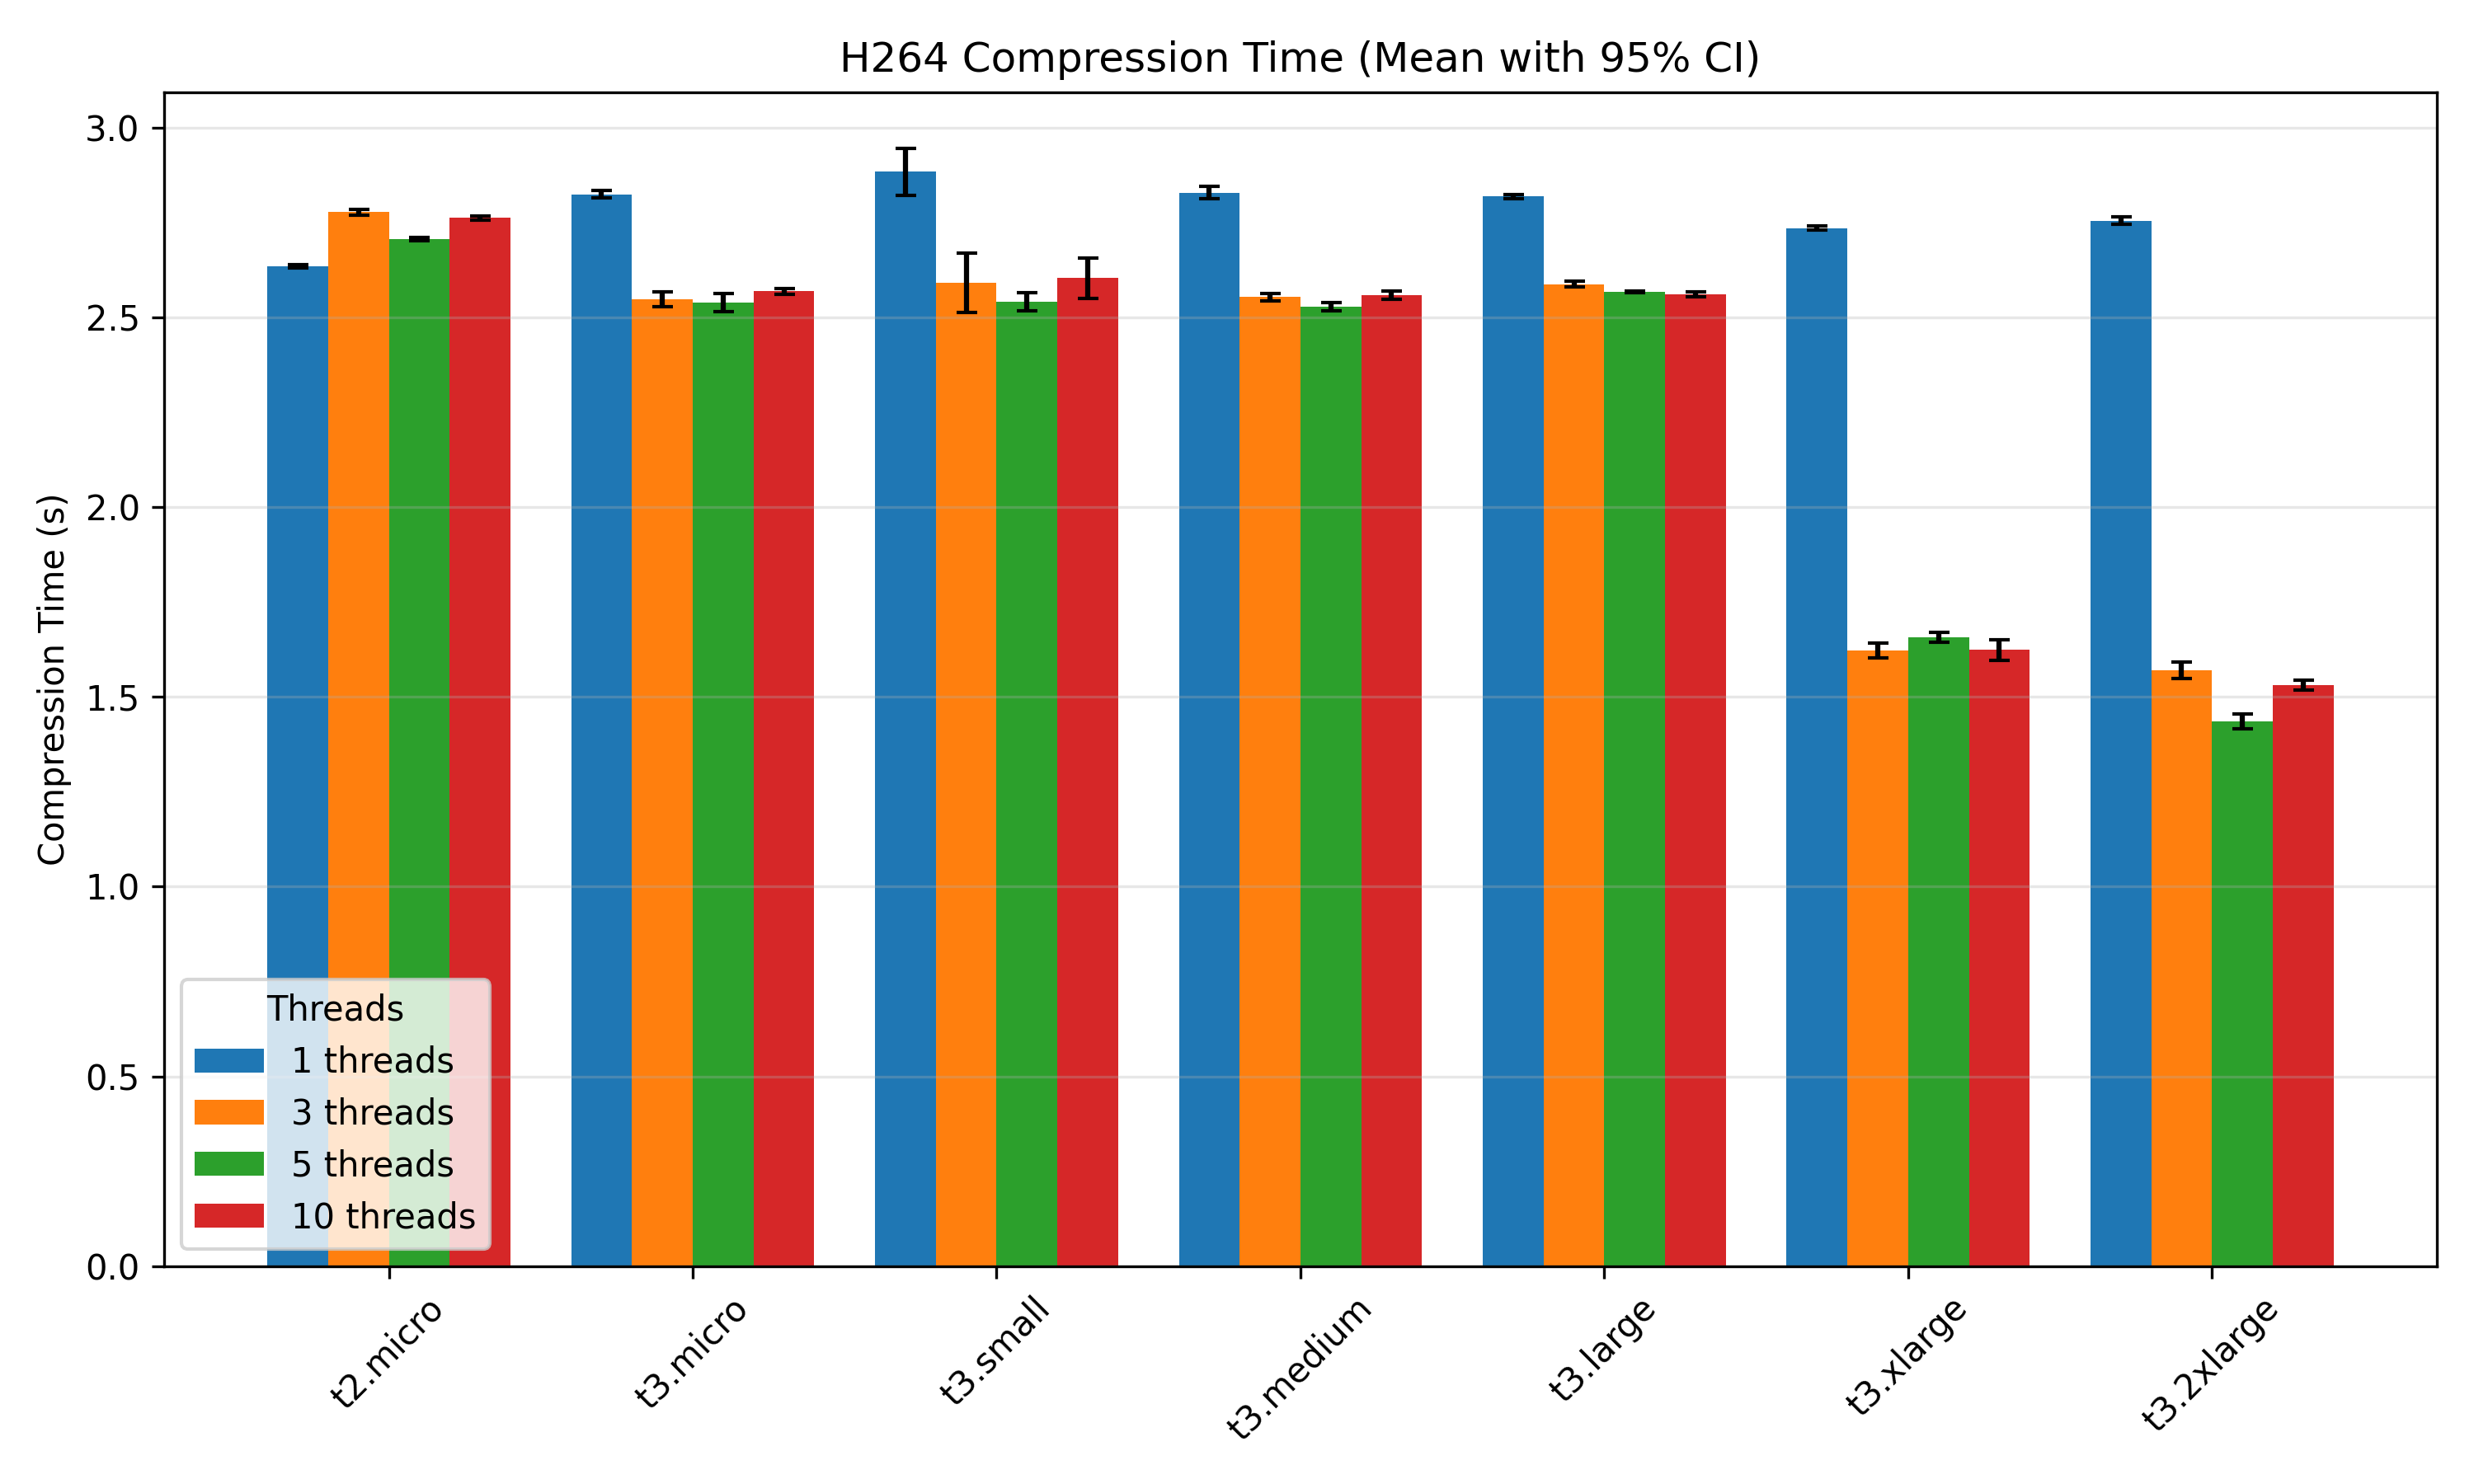
\includegraphics[width=\linewidth]{graphs/bar_chart_time_h264.png}
			\caption{H.264 Codec Performance}
			\label{fig:chart_h264}
		\end{subfigure}
		
		\vspace{0.5cm}
		
		\begin{subfigure}{\columnwidth}
			\centering
			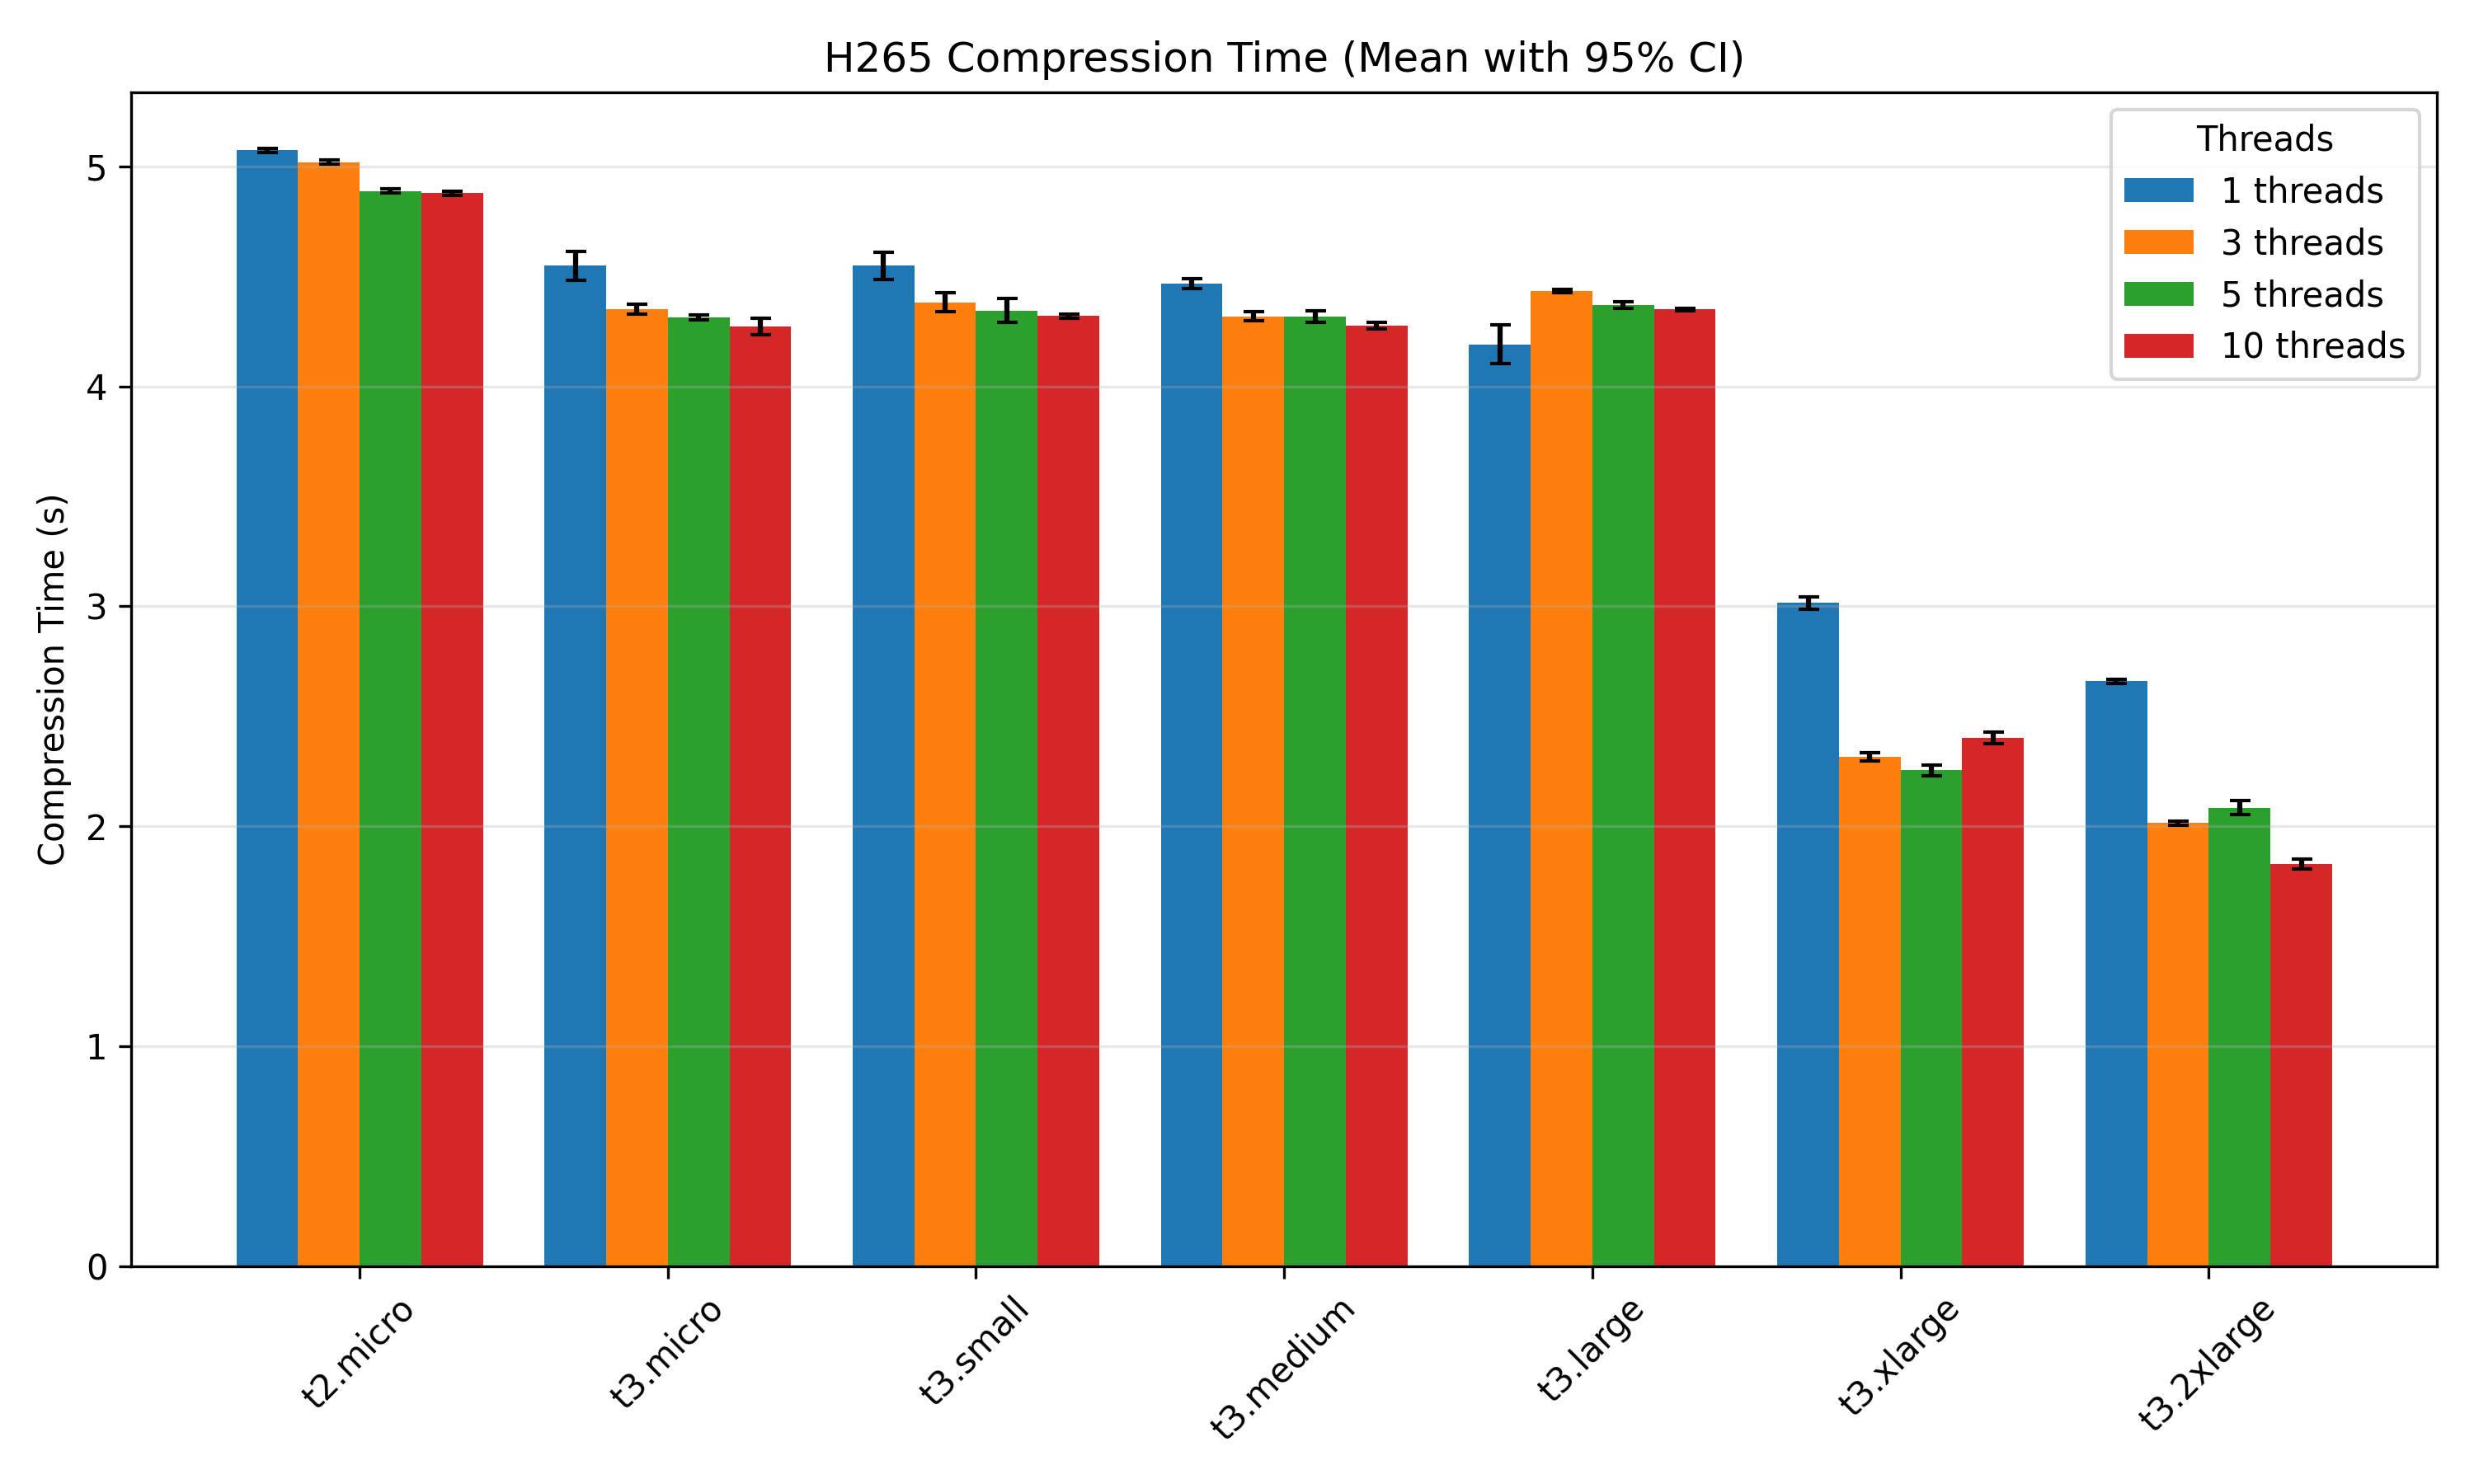
\includegraphics[width=\linewidth]{graphs/bar_chart_time_h265.png}
			\caption{H.265 Codec Performance}
			\label{fig:chart_h265}
		\end{subfigure}
		
		\vspace{0.5cm}
		
		\begin{subfigure}{\columnwidth}
			\centering
			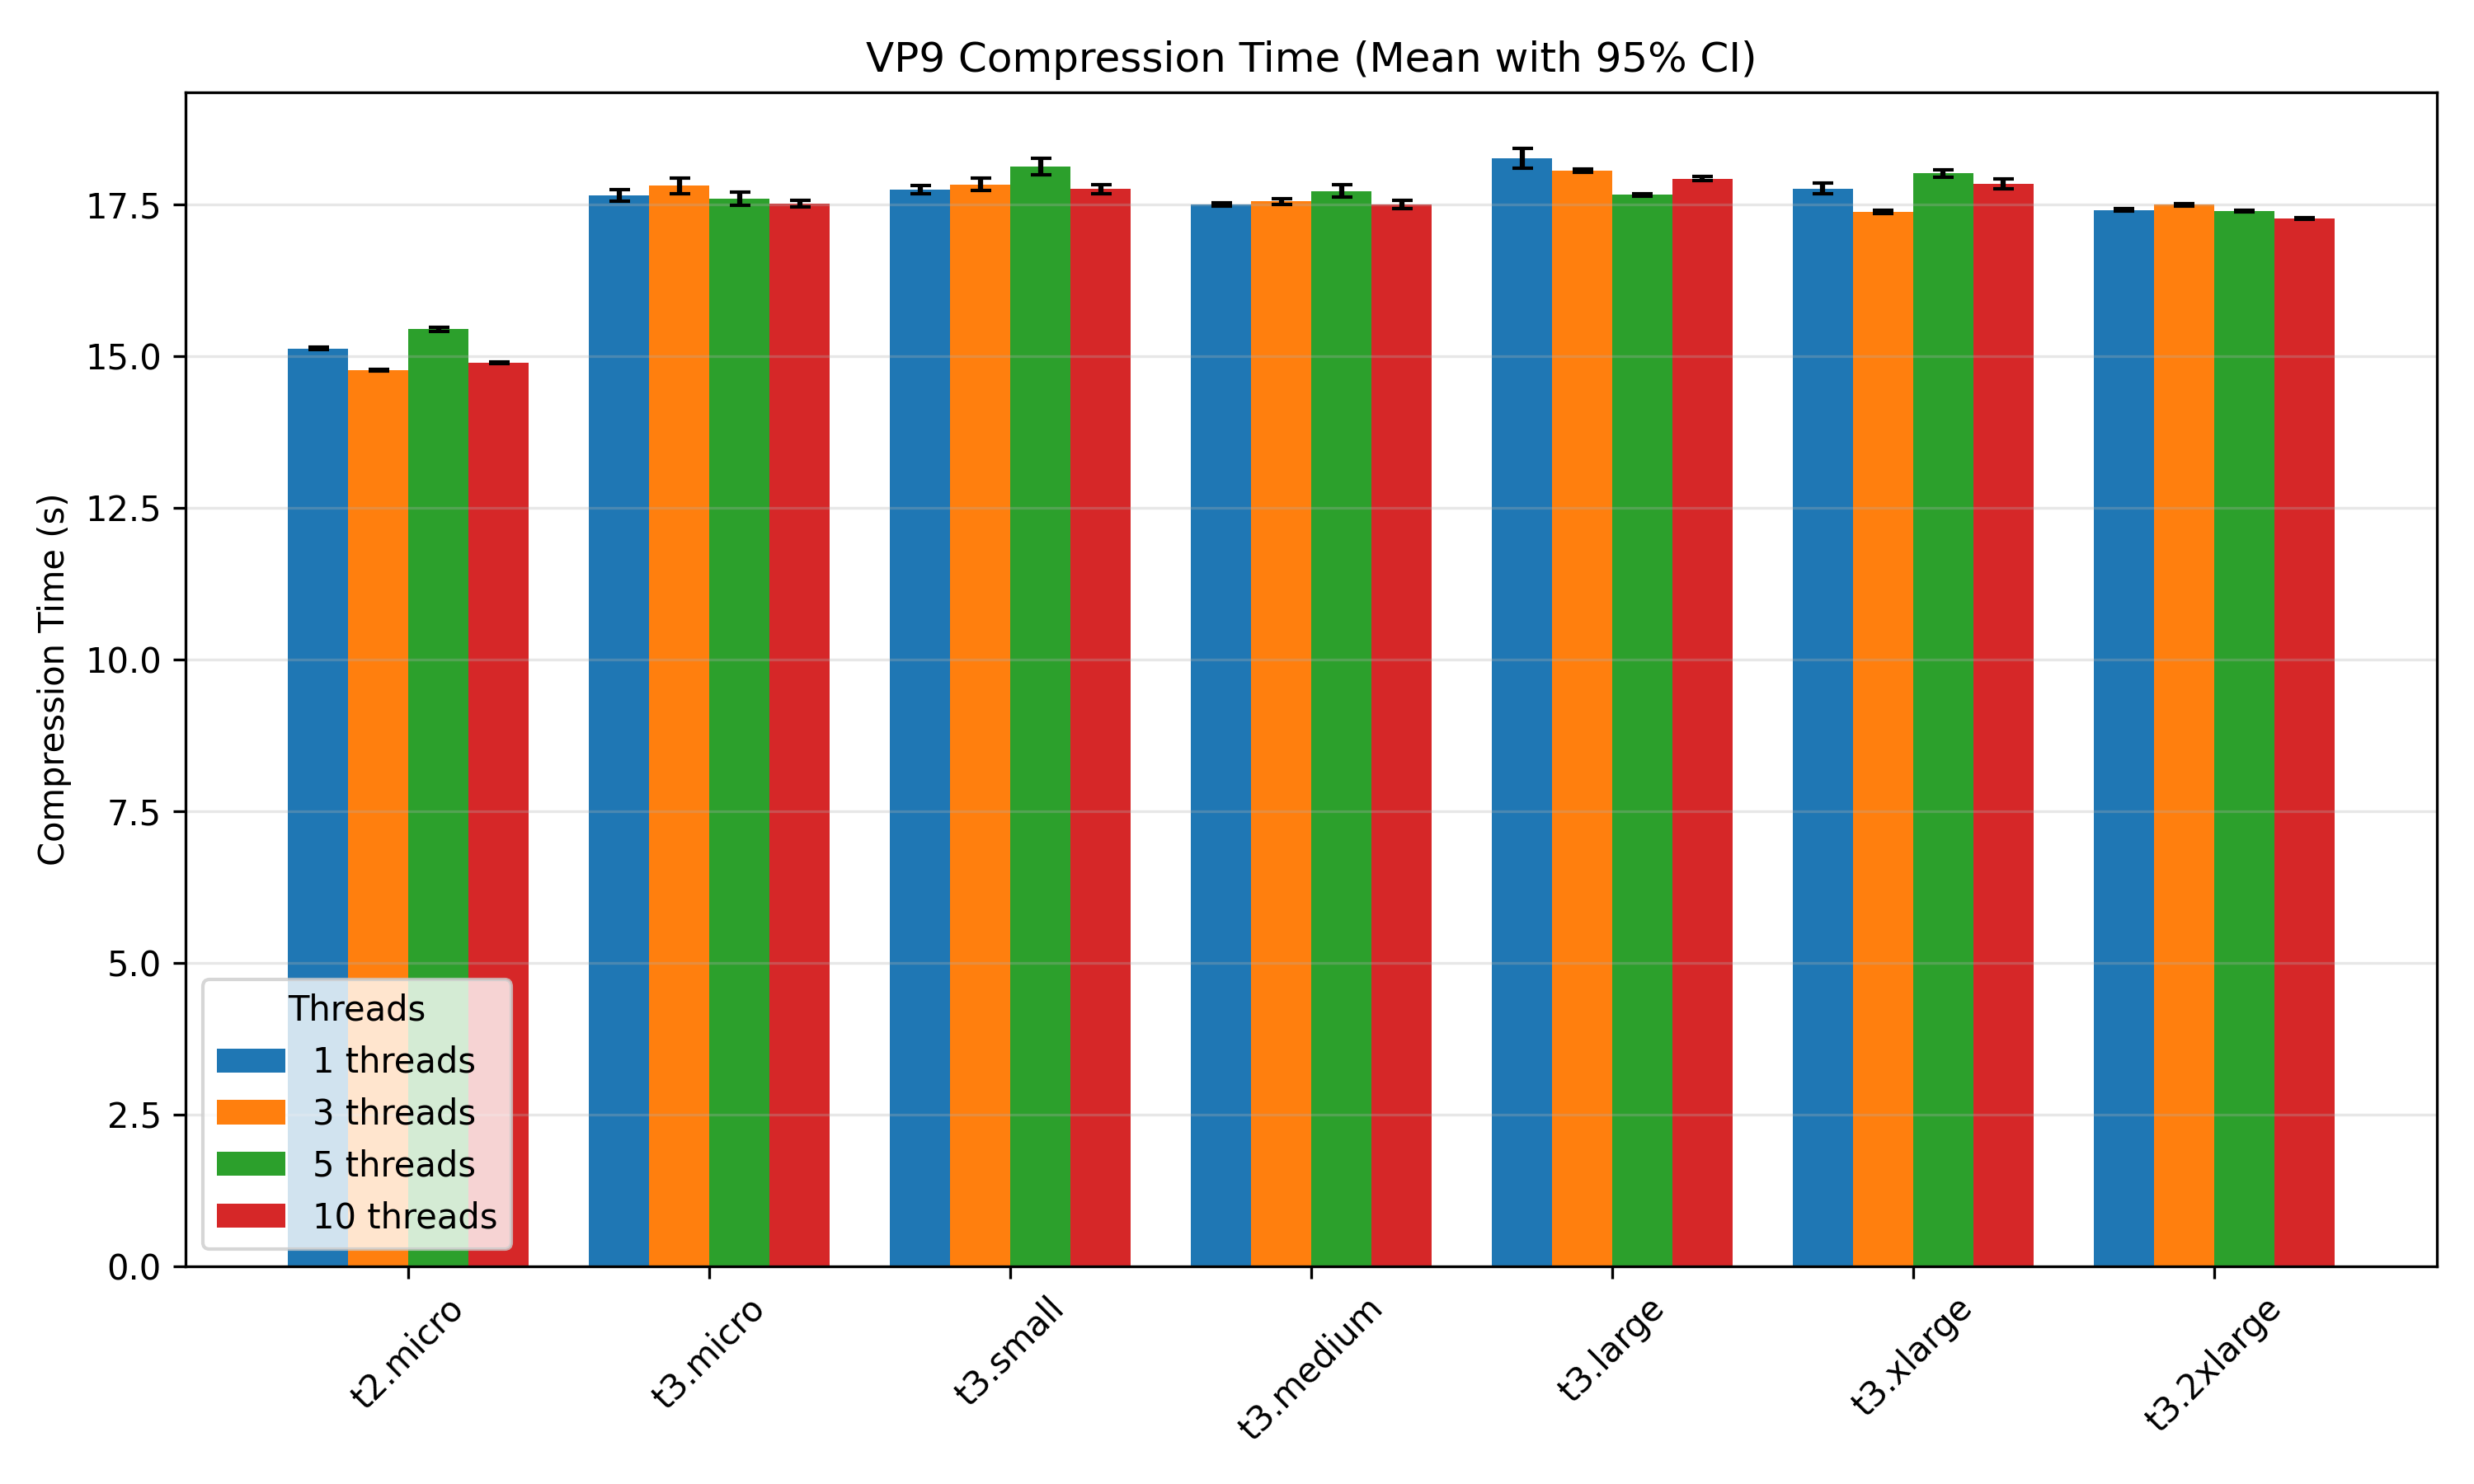
\includegraphics[width=\linewidth]{graphs/bar_chart_time_vp9.png}
			\caption{VP9 Codec Performance}
			\label{fig:chart_vp9}
		\end{subfigure}
		
		\caption{Comparative analysis of median compression time across instance configurations for (a) H.264, (b) H.265, and (c) VP9 codecs. Each panel illustrates performance scaling with varying thread counts, demonstrating distinct parallelization efficiency patterns across instance types.}
		\label{fig:faceted_bar_charts}
	\end{figure}
	
	\textbf{Hierarchical Efficiency Overview}
	Figure~\ref{fig:sunburst_efficiency_normalized_overall} presents a normalized Sunburst chart providing a hierarchical overview of encoding efficiency across all experimental configurations. The visualization comprises three independent segments representing H.264, H.265, and VP9 codecs, with efficiency values normalized within each segment. This approach enables clear comparison of instance and thread configurations within each algorithmic context, highlighting optimal setups for specific encoding tasks.
	
	\begin{figure*}[ht]
		\centering
		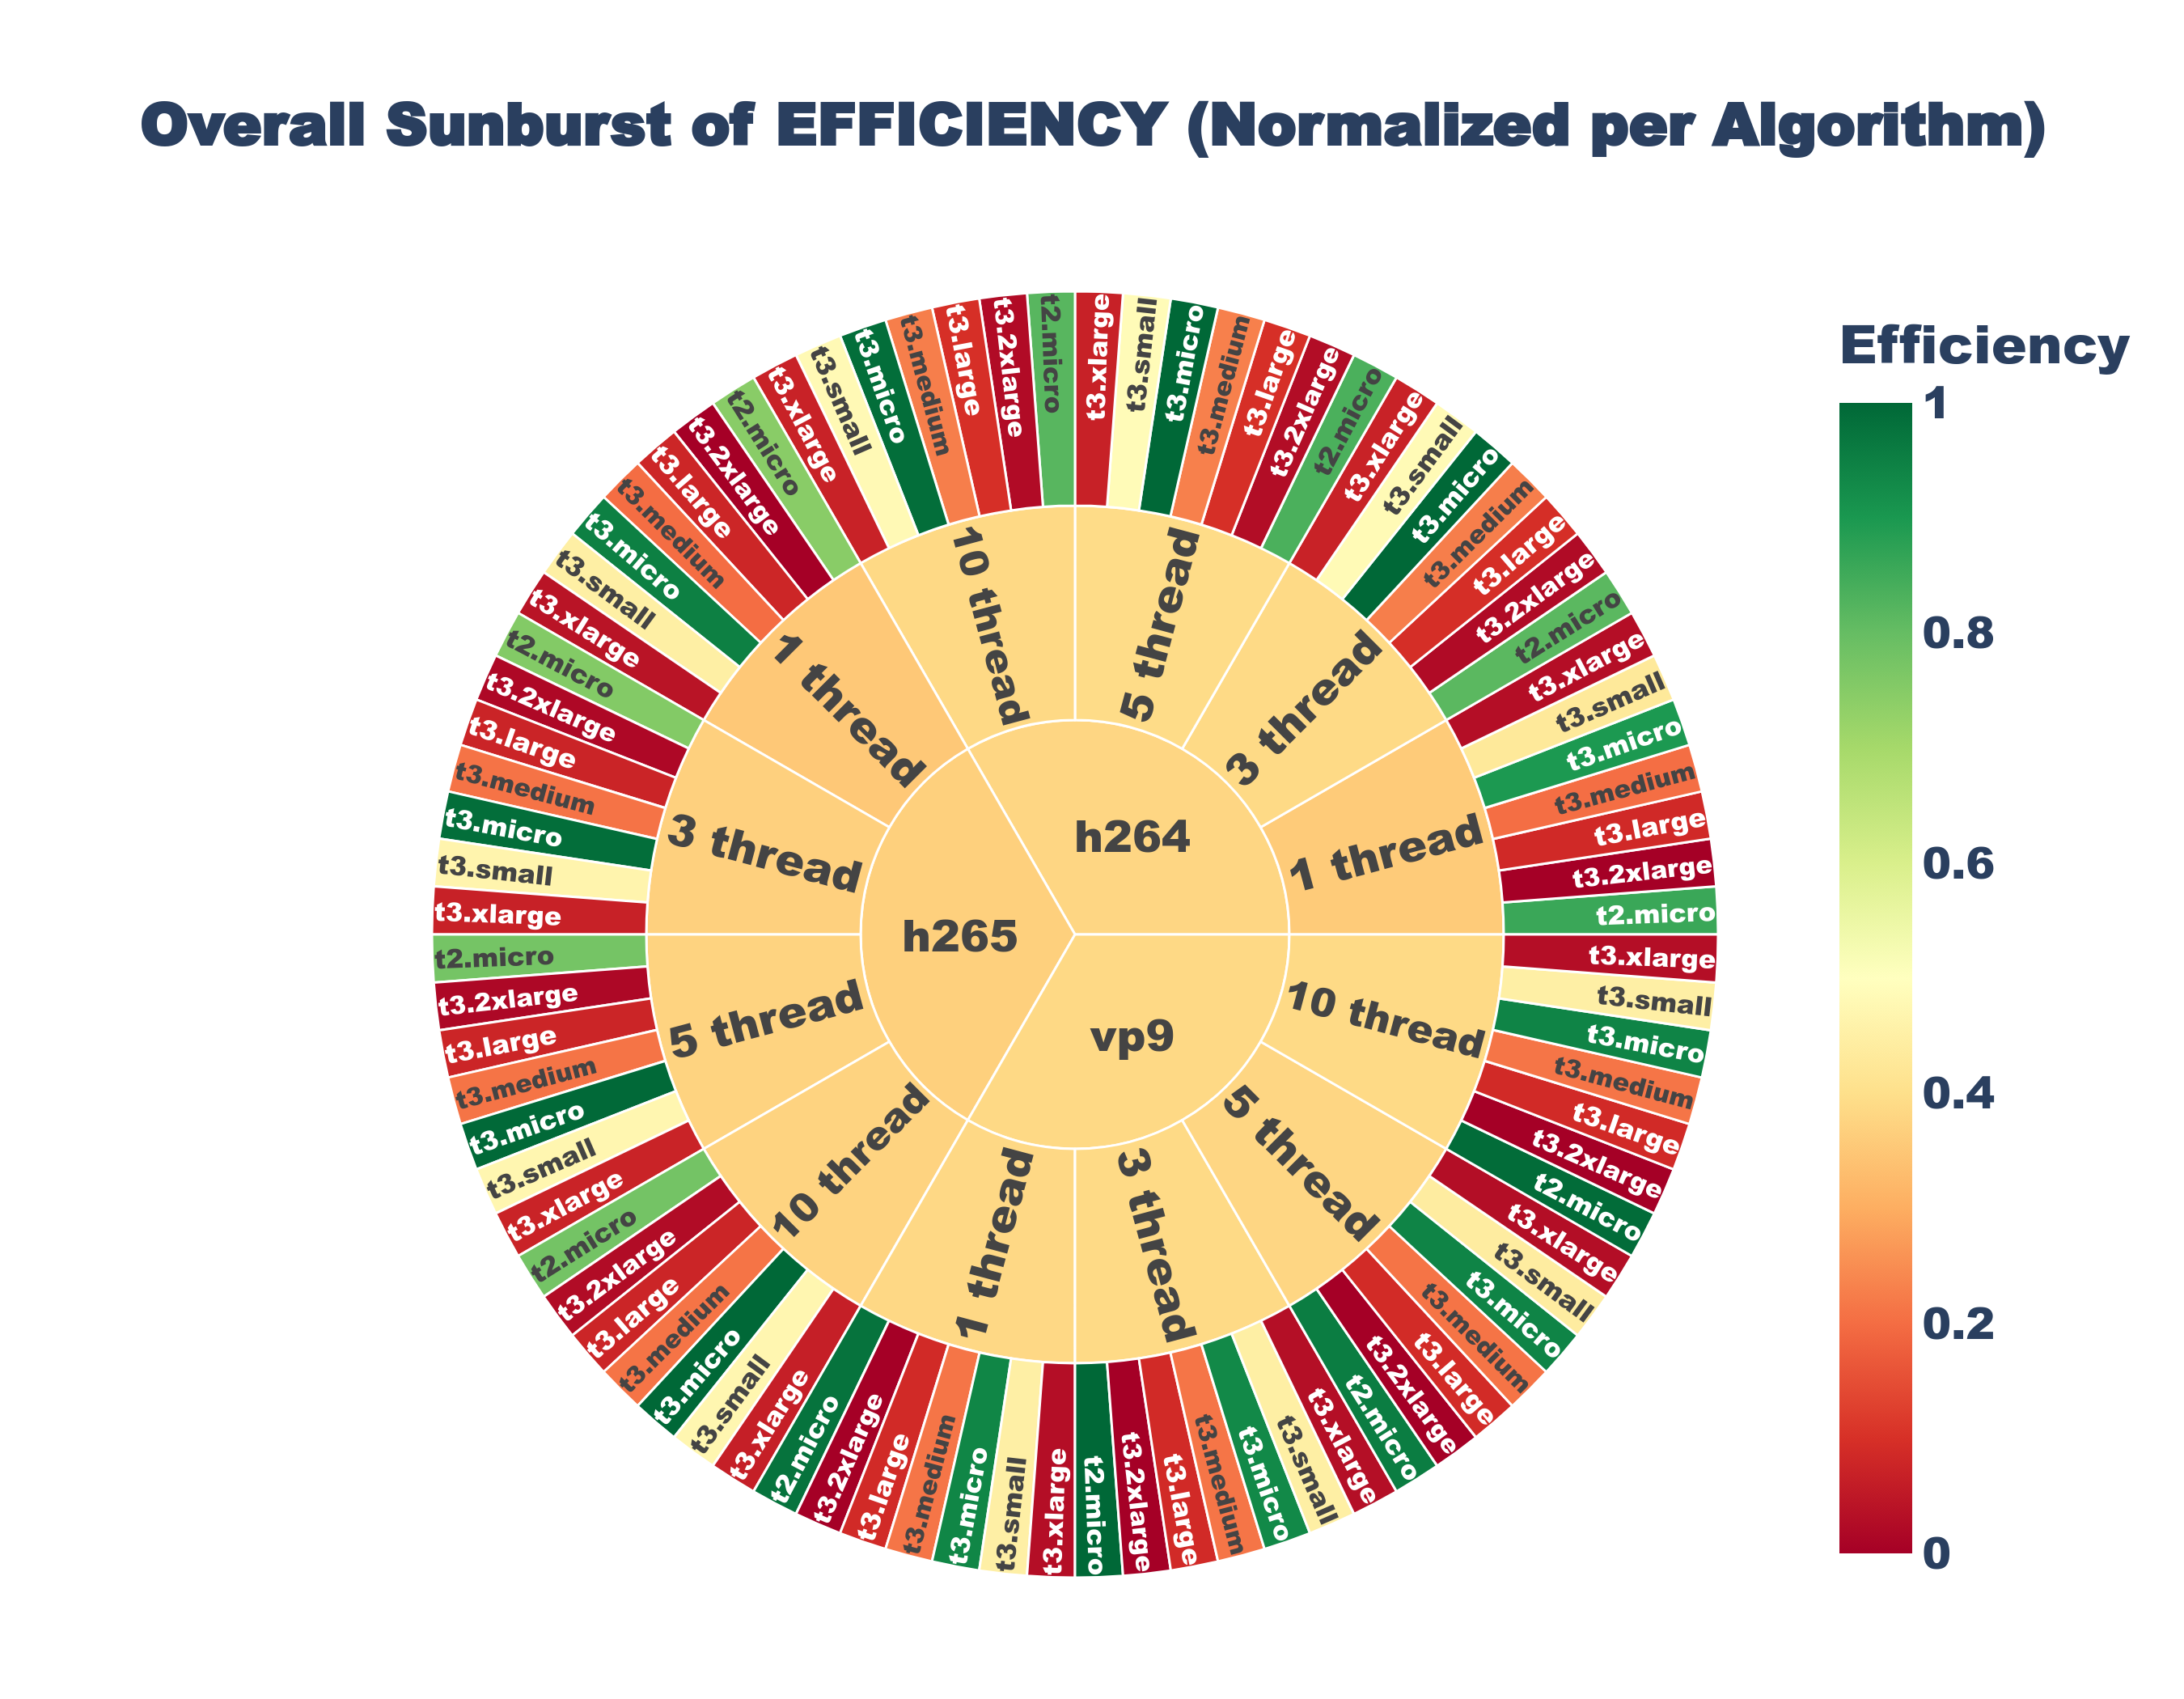
\includegraphics[width=0.7\textwidth]{graphs/sunburst_efficiency_normalized_overall.pdf}
		\caption{Hierarchical visualization of encoding efficiency across all experimental configurations. The sunburst diagram organizes results by codec family (outer ring), thread count (middle ring), and instance type (inner segments), with color intensity and segment size proportional to normalized efficiency values within each algorithmic category.}
		\label{fig:sunburst_efficiency_normalized_overall}
	\end{figure*}
	
	\textbf{Algorithm-Specific Efficiency Analysis}
	Figure~\ref{fig:heatmaps_efficiency} presents a series of heatmaps visualizing median efficiency for each algorithm individually. Each heatmap correlates thread count with instance type, with color intensity representing cost-efficiency. This approach enables straightforward identification of optimal configurations (the "sweet spot") for specific codecs, answering the practical question of which instance and thread count combination yields maximum efficiency for given encoding tasks.
	
	\begin{figure}[htpb]
		\centering
		\begin{subfigure}{\columnwidth}
			\centering
			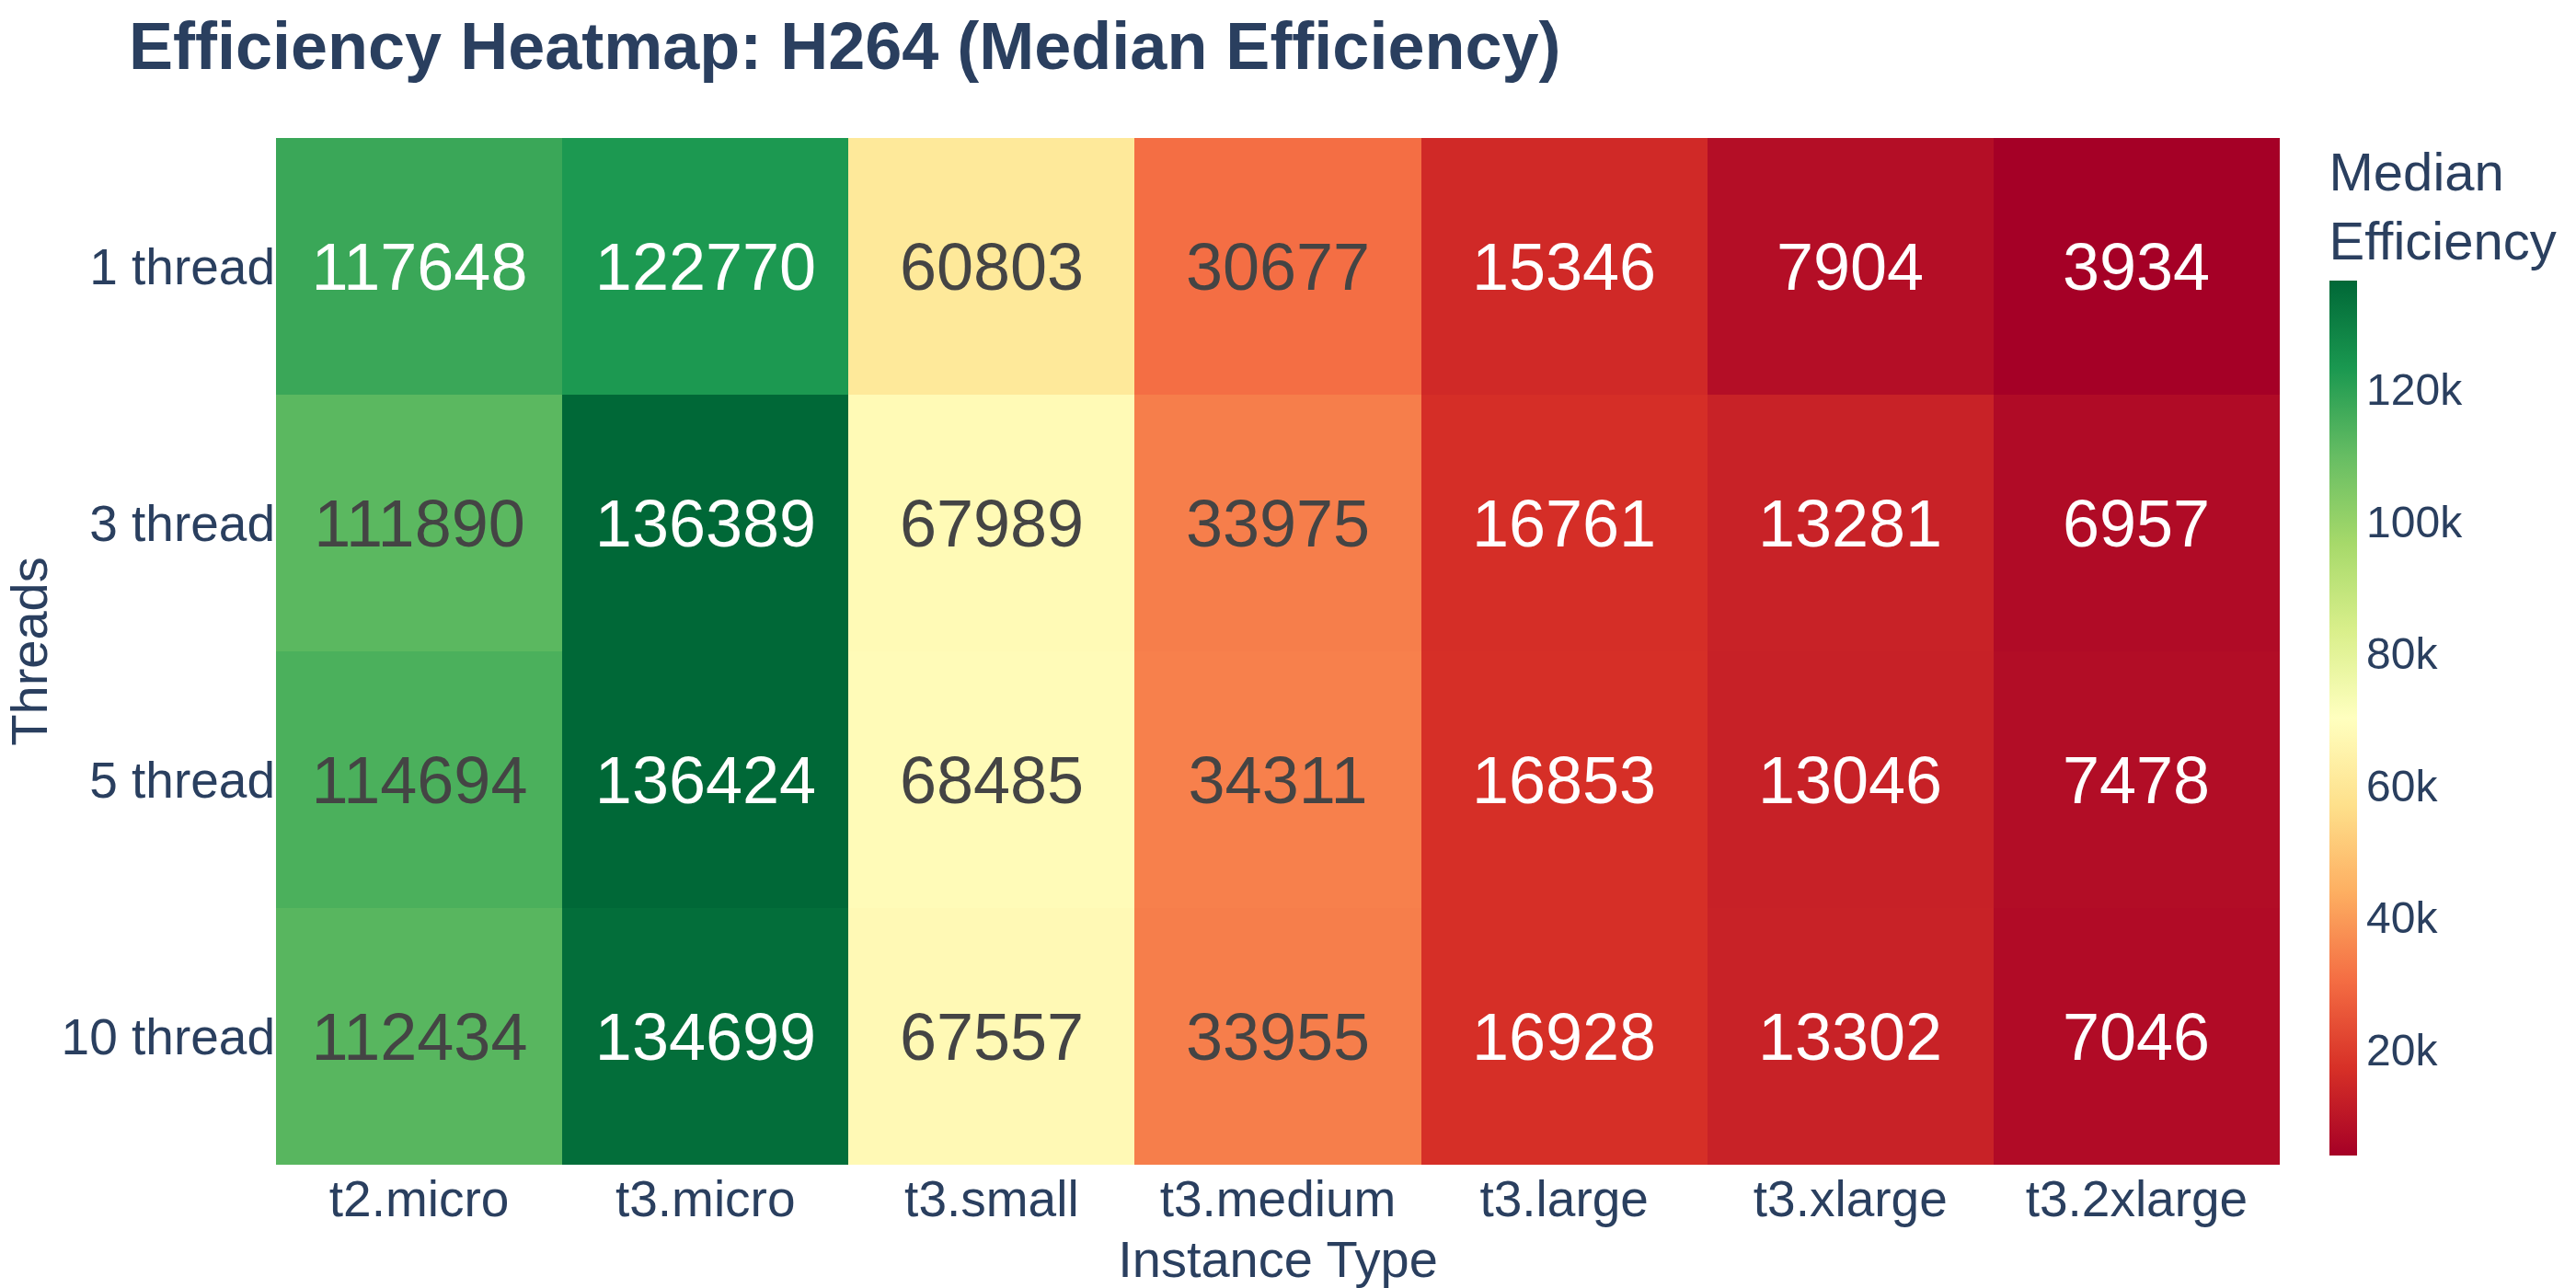
\includegraphics[width=0.98\columnwidth,height=5cm,keepaspectratio]{graphs/heatmap_efficiency_h264.png}
			\caption{H.264 Codec Efficiency}
			\label{fig:h264}
		\end{subfigure}
		\vfill
		\begin{subfigure}{\columnwidth}
			\centering
			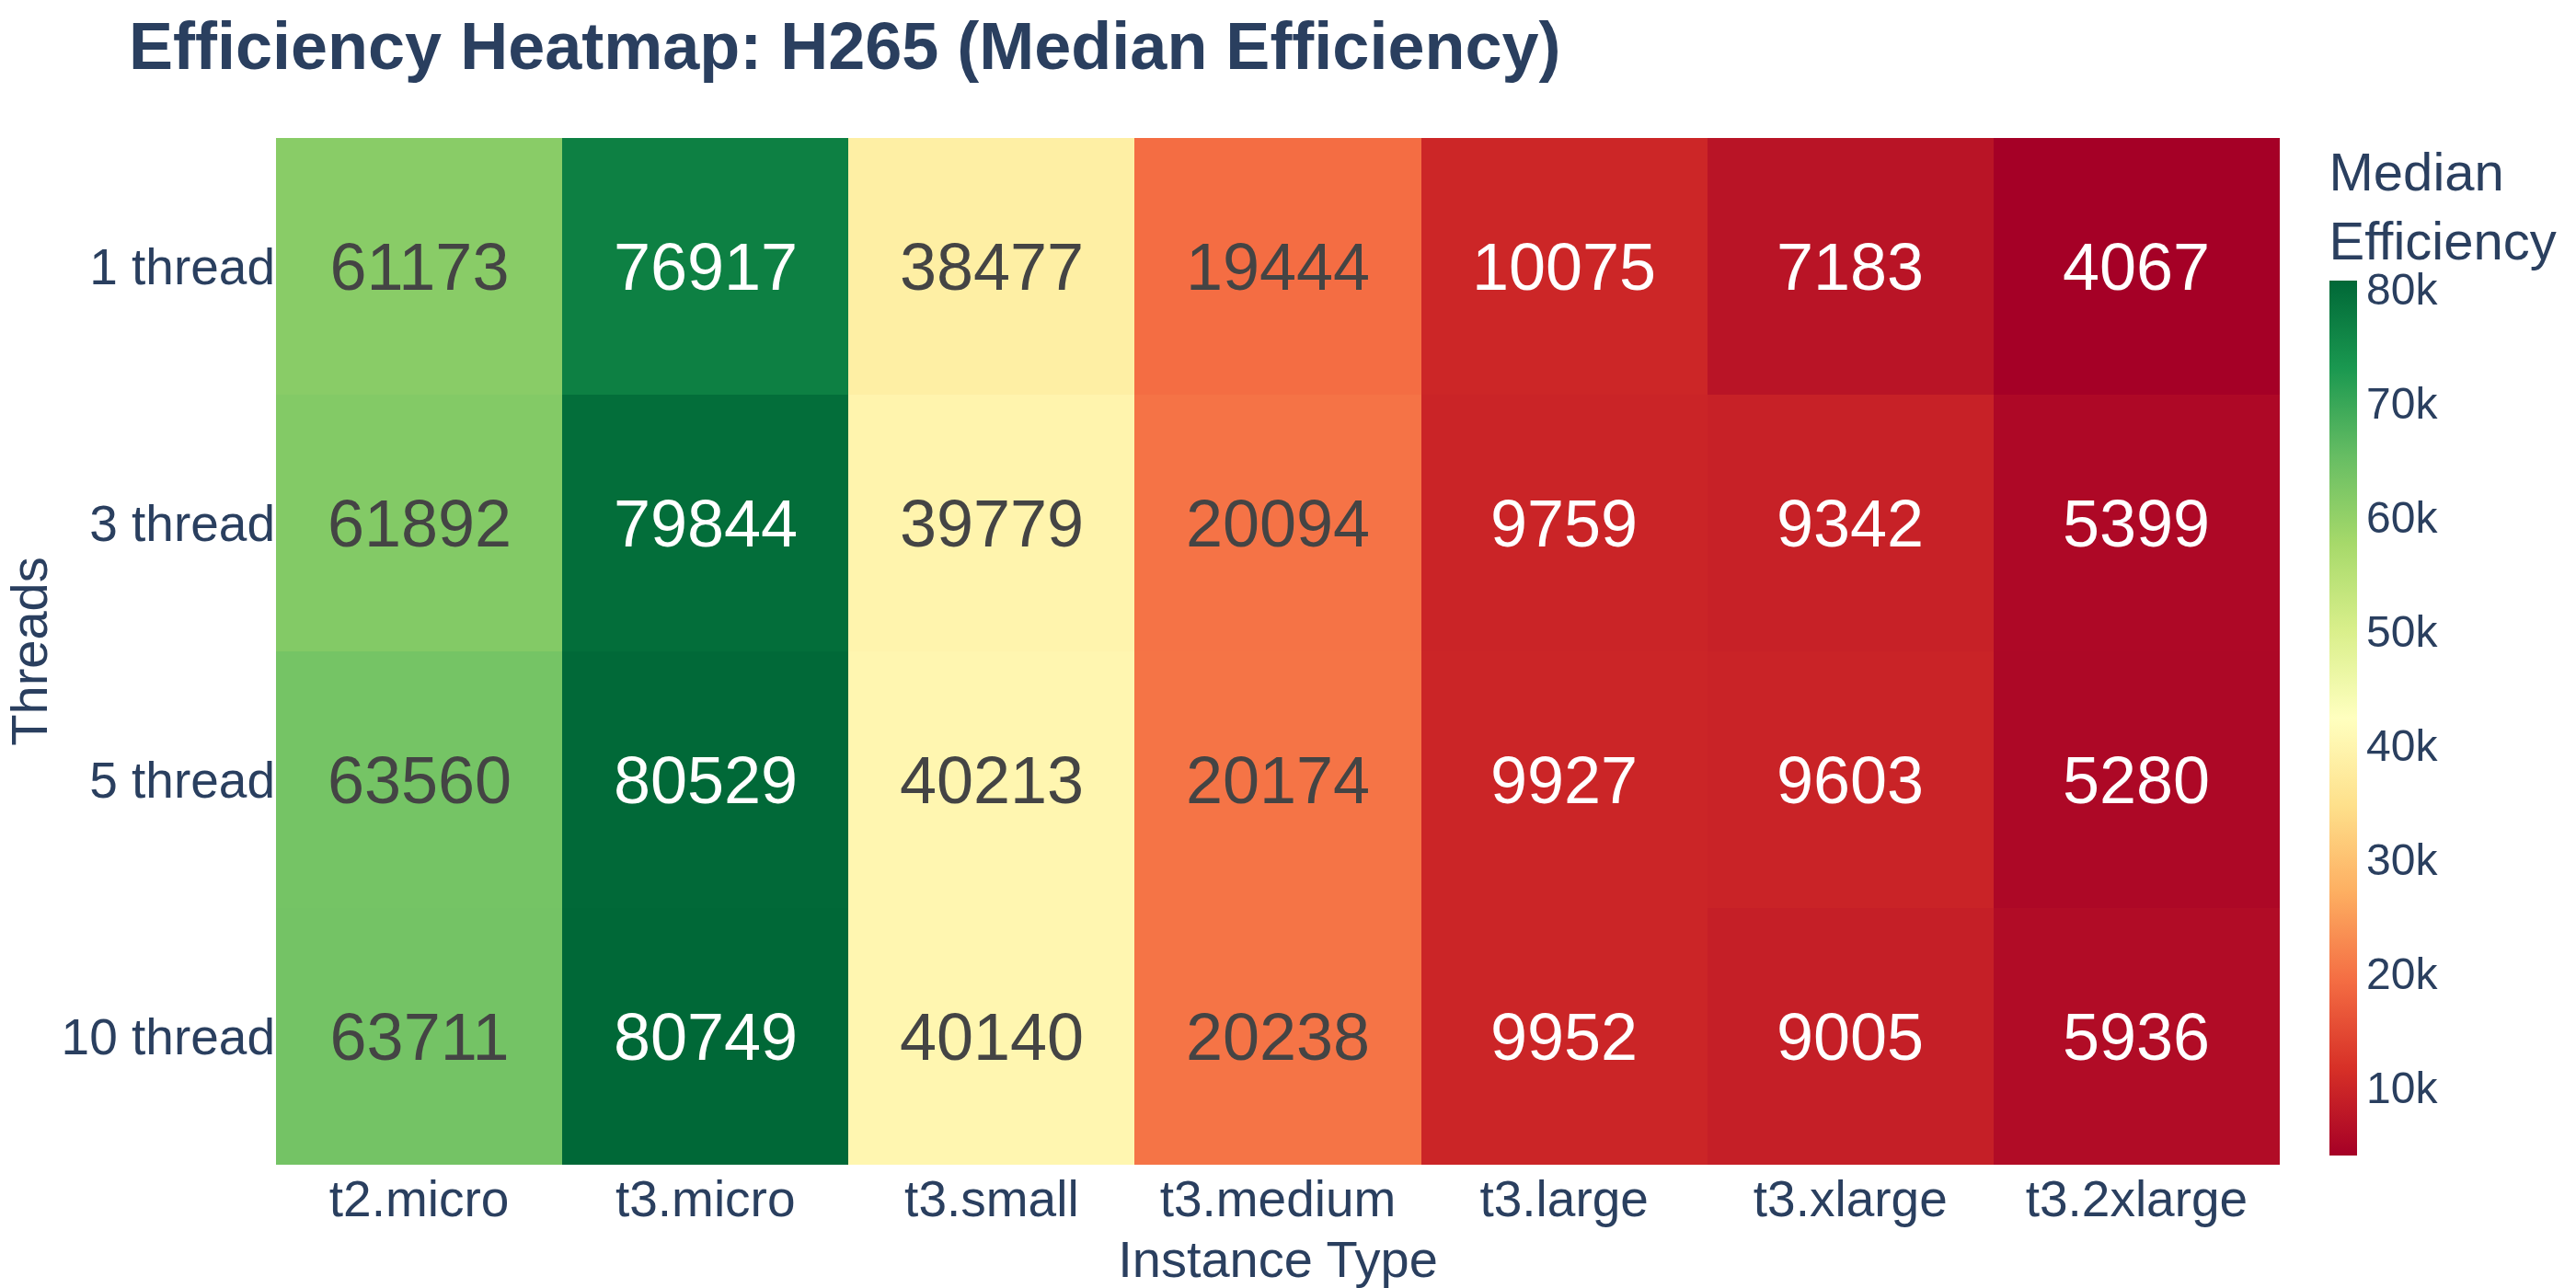
\includegraphics[width=0.98\columnwidth,height=5cm,keepaspectratio]{graphs/heatmap_efficiency_h265.png}
			\caption{H.265 Codec Efficiency}
			\label{fig:h265}
		\end{subfigure}
		\vfill
		\begin{subfigure}{\columnwidth}
			\centering
			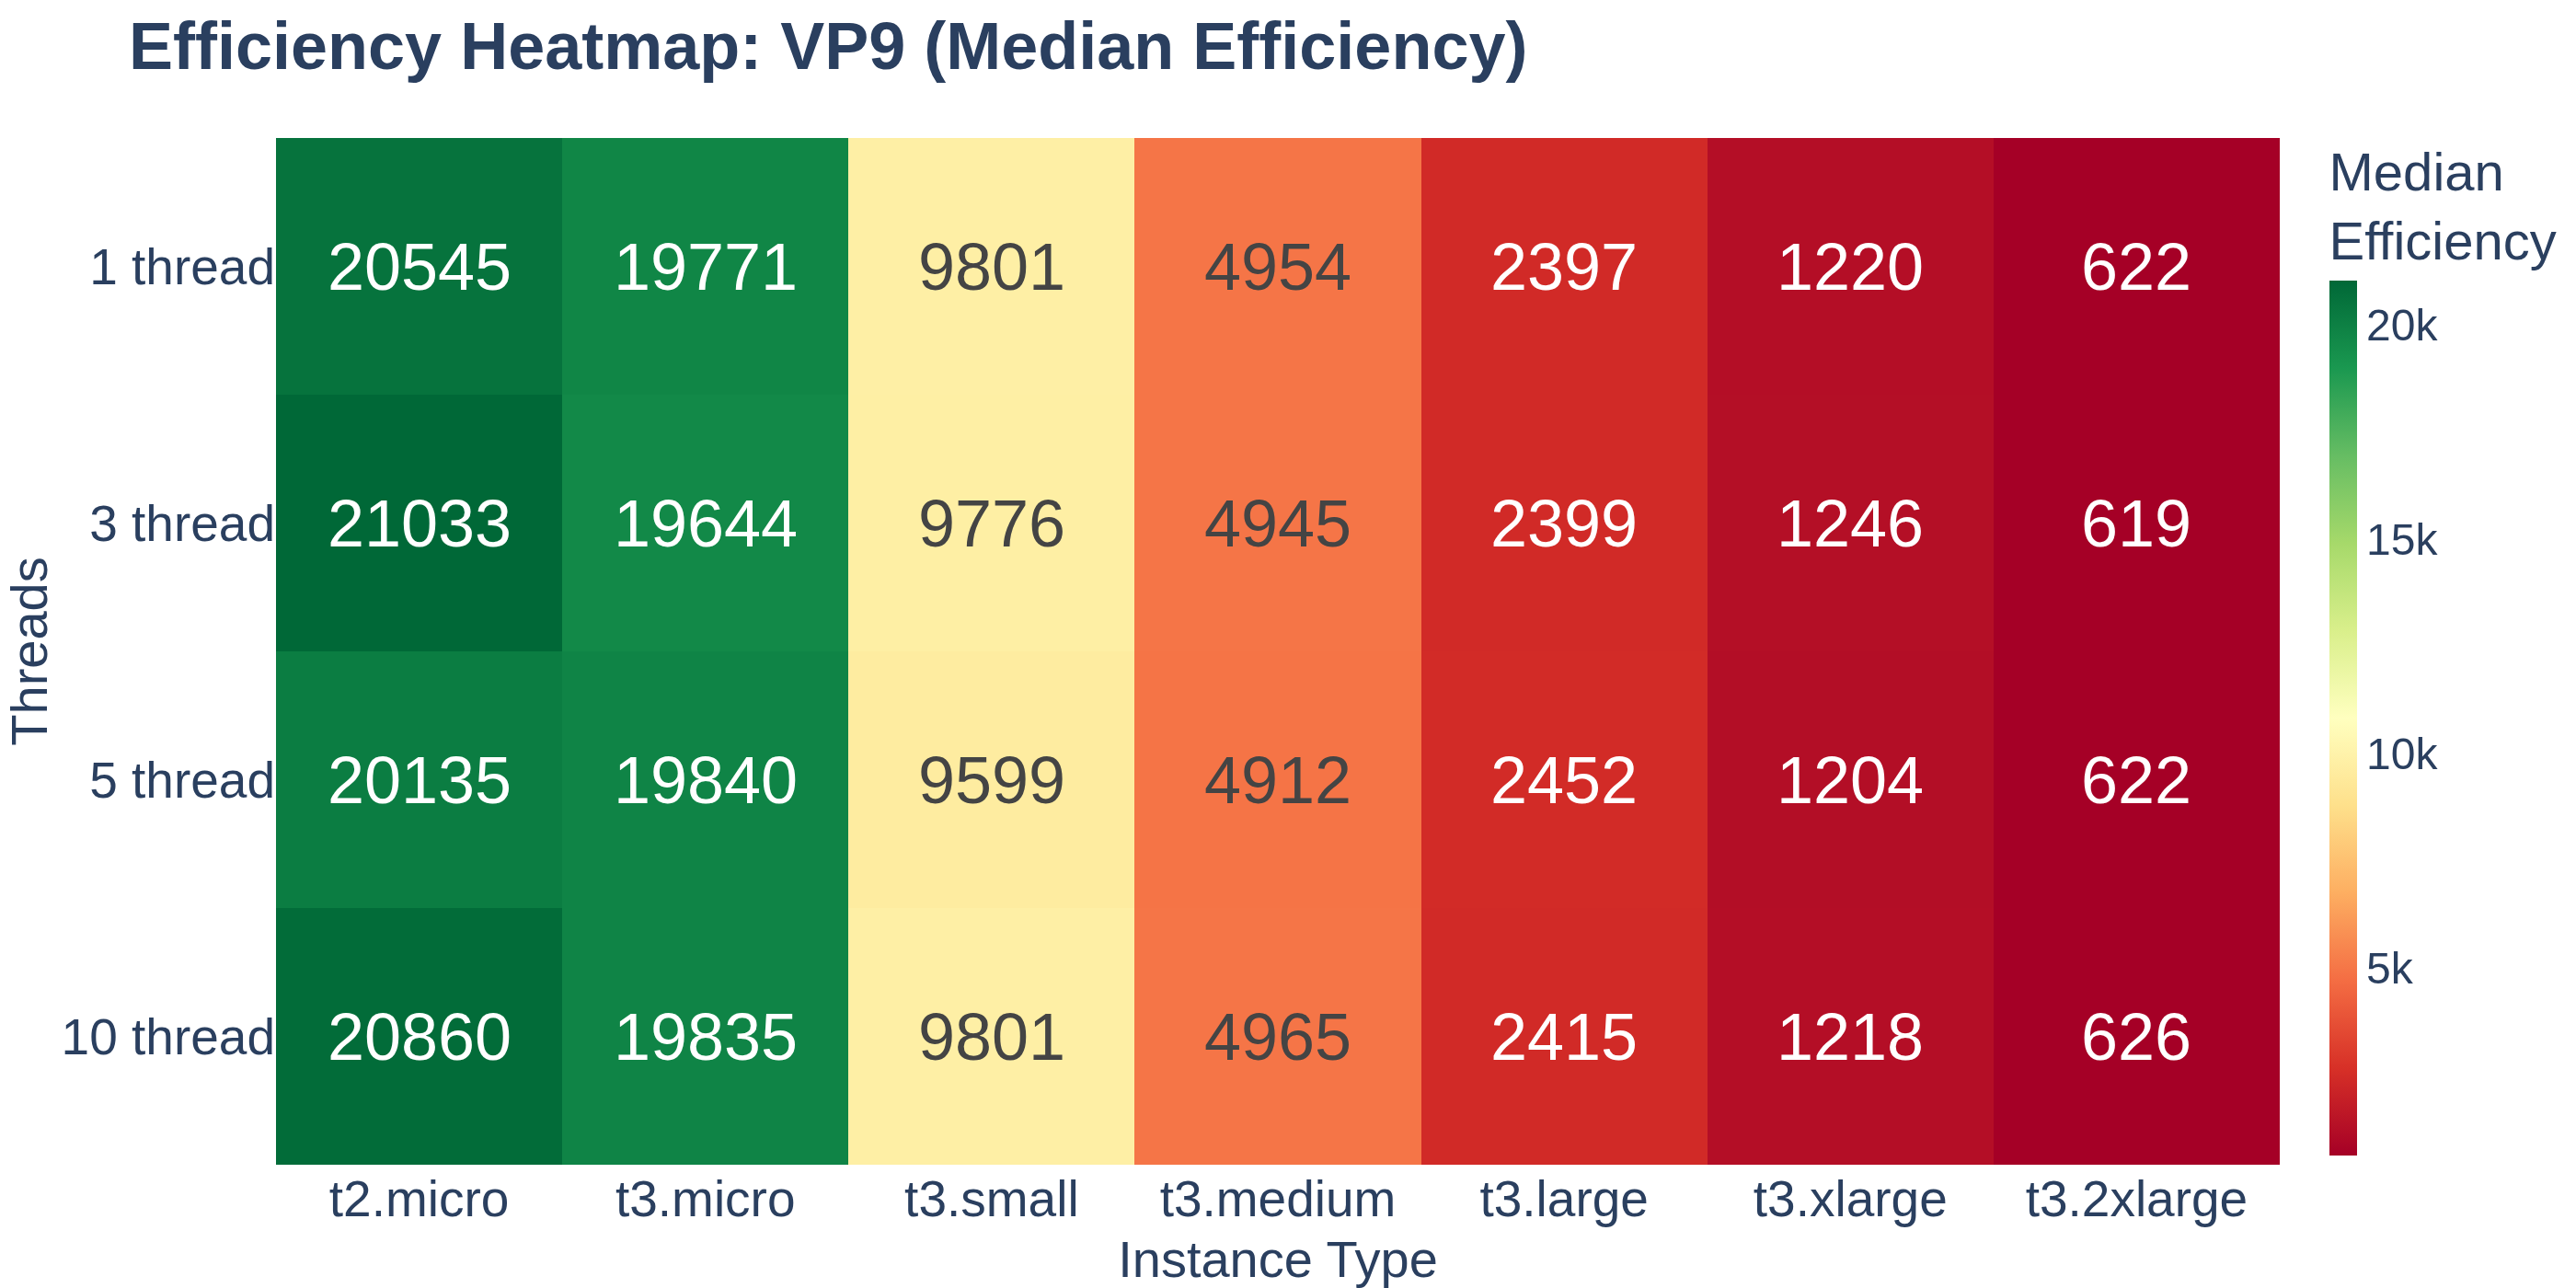
\includegraphics[width=0.98\columnwidth,height=5cm,keepaspectratio]{graphs/heatmap_efficiency_vp9.png}
			\caption{VP9 Codec Efficiency}
			\label{fig:vp9}
		\end{subfigure}
		\caption{Algorithm-specific efficiency analysis through heatmap visualization for (a) H.264, (b) H.265, and (c) VP9 codecs. Each heatmap correlates thread count (vertical axis) with instance type (horizontal axis), with color intensity representing cost-efficiency. Optimal configurations emerge as regions of maximum intensity.}
		\label{fig:heatmaps_efficiency}
	\end{figure}
	
	\subsection{Phase 3 Results: Horizontal vs. Vertical Scaling Analysis}
	\label{results-phase3}
	
	Based on initial findings identifying \texttt{t3.micro} as the most cost-effective for H.264 compression, we compared horizontal and vertical scaling strategies for video encoding workloads to determine if clusters of cost-efficient instances outperform single powerful instances.
	
	\subsubsection{Experimental Design and Methodology}
	
	The scaling analysis employed a structured two-phase approach to isolate and quantify the impact of provisioning overhead, representing a significant methodological contribution to cloud performance evaluation:
	
	\begin{itemize}
		\item \textbf{Workload:} 10-minute high-resolution video file representing a realistic encoding task
		\item \textbf{Horizontal Scaling:} 10 \texttt{t3.micro} instances (2 vCPUs, 1 GiB RAM each) processing one-minute segments in parallel
		\item \textbf{Vertical Scaling:} Single \texttt{t3.2xlarge} instance (8 vCPUs, 32 GiB RAM) processing complete video as integrated workload
		\item \textbf{Baseline:} Single \texttt{t3.micro} instance processing video sequentially to establish performance baseline
		\item \textbf{Methodological Innovation:} Two-phase design isolating provisioning overhead from core computational performance
	\end{itemize}
	
	\subsubsection{Phase 3.1: Dynamic Provisioning Results}
	
	The initial phase employed dynamic provisioning with standard Ubuntu images and post-deployment dependency installation, representing typical cloud deployment patterns. As detailed in Table~\ref{tab:unified_case_study}, this approach quantified operational overhead that impacts scaling efficiency:
	
	\begin{itemize}
		\item \textbf{Provisioning Overhead Dominance:} Setup activities consumed 56.1-75.9\% of total processing time across all configurations, with parallel architectures suffering the highest overhead (70.2\%). This finding challenges assumptions that computational performance alone determines scaling efficiency.
		
		\item \textbf{Raw Performance Comparison:} In the initial phase with dynamic provisioning, the vertical scaling approach completed the workload in 3.04 minutes, outperforming the horizontal scaling approach (3.28 minutes) by approximately 7.9%. This indicates that without optimization, the overhead of parallelization can negate the benefits of distributed processing.
		
		\item \textbf{Cost Analysis:} Despite the performance disadvantage in the unoptimized phase, the horizontal approach demonstrated significant cost advantages, incurring only \$0.00568 compared to \$0.01687 for vertical scaling—a 66.3\% reduction. This cost-effectiveness persists even with provisioning overhead, though optimization potential remains substantial.
	\end{itemize}
	
	\subsubsection{Phase 3.2: Optimized Provisioning Results}
	
	The identification of provisioning overhead as the primary bottleneck motivated Phase 3.2, which employed custom Amazon Machine Images (AMIs) with pre-installed dependencies. This optimization yielded transformative results that fundamentally alter the scaling strategy calculus:
	\begin{itemize}
		\item \textbf{Performance Improvements:} The horizontal scaling approach achieved \textbf{1.45 minutes} total processing time—a \textbf{55.9\% improvement} over Phase 3.1 and \textbf{1.28× faster} than vertical scaling (1.85 minutes).
		
		\item \textbf{Cost Reduction:} Optimized horizontal scaling reduced costs by \textbf{55.8\%} to \$0.00251, achieving \textbf{75.5\% cost reduction} compared to vertical scaling.
		
		\item \textbf{Overhead Elimination:} Setup time decreased from 2.30 minutes to 0.98 minutes in the horizontal configuration, representing a \textbf{57.4\% reduction} in absolute setup time. While overhead as a percentage of total time decreased from 70.2\% to 67.6\%, the reduction in absolute setup time was crucial for overall performance gains.
	\end{itemize}
	
	\subsubsection{Comprehensive Analysis and Validation}
	
	The two-phase analysis shows that properly optimized horizontal scaling achieves better performance and cost-efficiency, with experimental data revealing::
	
	\begin{table*}[t]
		\centering
		\caption{Comprehensive comparison of scaling strategies across optimization phases}
		\label{tab:unified_case_study}
		\begin{tabular*}{\textwidth}{l @{\extracolsep{\fill}} | cc | cc | cc}
			\toprule
			& \multicolumn{2}{c|}{\textbf{Serial (1x t3.micro)}} & \multicolumn{2}{c|}{\textbf{Parallel (10x t3.micro)}} & \multicolumn{2}{c}{\textbf{Serial (1x t3.2xlarge)}} \\
			\cmidrule(lr){2-3} \cmidrule(lr){4-5} \cmidrule(lr){6-7}
			\textbf{Metric} & \textbf{Phase 3.1} & \textbf{Phase 3.2} & \textbf{Phase 3.1} & \textbf{Phase 3.2} & \textbf{Phase 3.1} & \textbf{Phase 3.2} \\
			\midrule
			Total Time (min)          & 4.03  & 2.80  & 3.28 & \textbf{1.45} & 3.04 & 1.85 \\
			Setup Overhead (min)      & 2.26  & 1.02  & 2.30 & \textbf{0.98} & 2.31 & 1.11 \\
			Setup Overhead (\%)       & 56.1\% & 36.5\% & 70.2\% & 67.6\% & 75.9\% & 59.7\% \\
			Effective Encoding Time (min) & 1.77  & 1.78  & 0.97 & 0.47 & \textbf{0.73} & 0.74 \\
			\midrule
			Total Cost (USD)          & \$0.00070 & \$0.00048 & \$0.00568 & \textbf{\$0.00251} & \$0.01687 & \$0.01026 \\
			Cost per Minute Video     & \$0.000070 & \$0.000048 & \$0.000568 & \textbf{\$0.000251} & \$0.001687 & \$0.001026 \\
			\midrule \midrule
			\textbf{Time Improvement} & \multicolumn{2}{c|}{30.5\%} & \multicolumn{2}{c|}{\textbf{55.9\%}} & \multicolumn{2}{c}{39.1\%} \\
			\textbf{Cost Reduction}   & \multicolumn{2}{c|}{31.4\%} & \multicolumn{2}{c|}{\textbf{55.8\%}} & \multicolumn{2}{c}{39.2\%} \\
			\bottomrule
		\end{tabular*}
	\end{table*}
	
	\begin{figure}[ht]
		\centering
		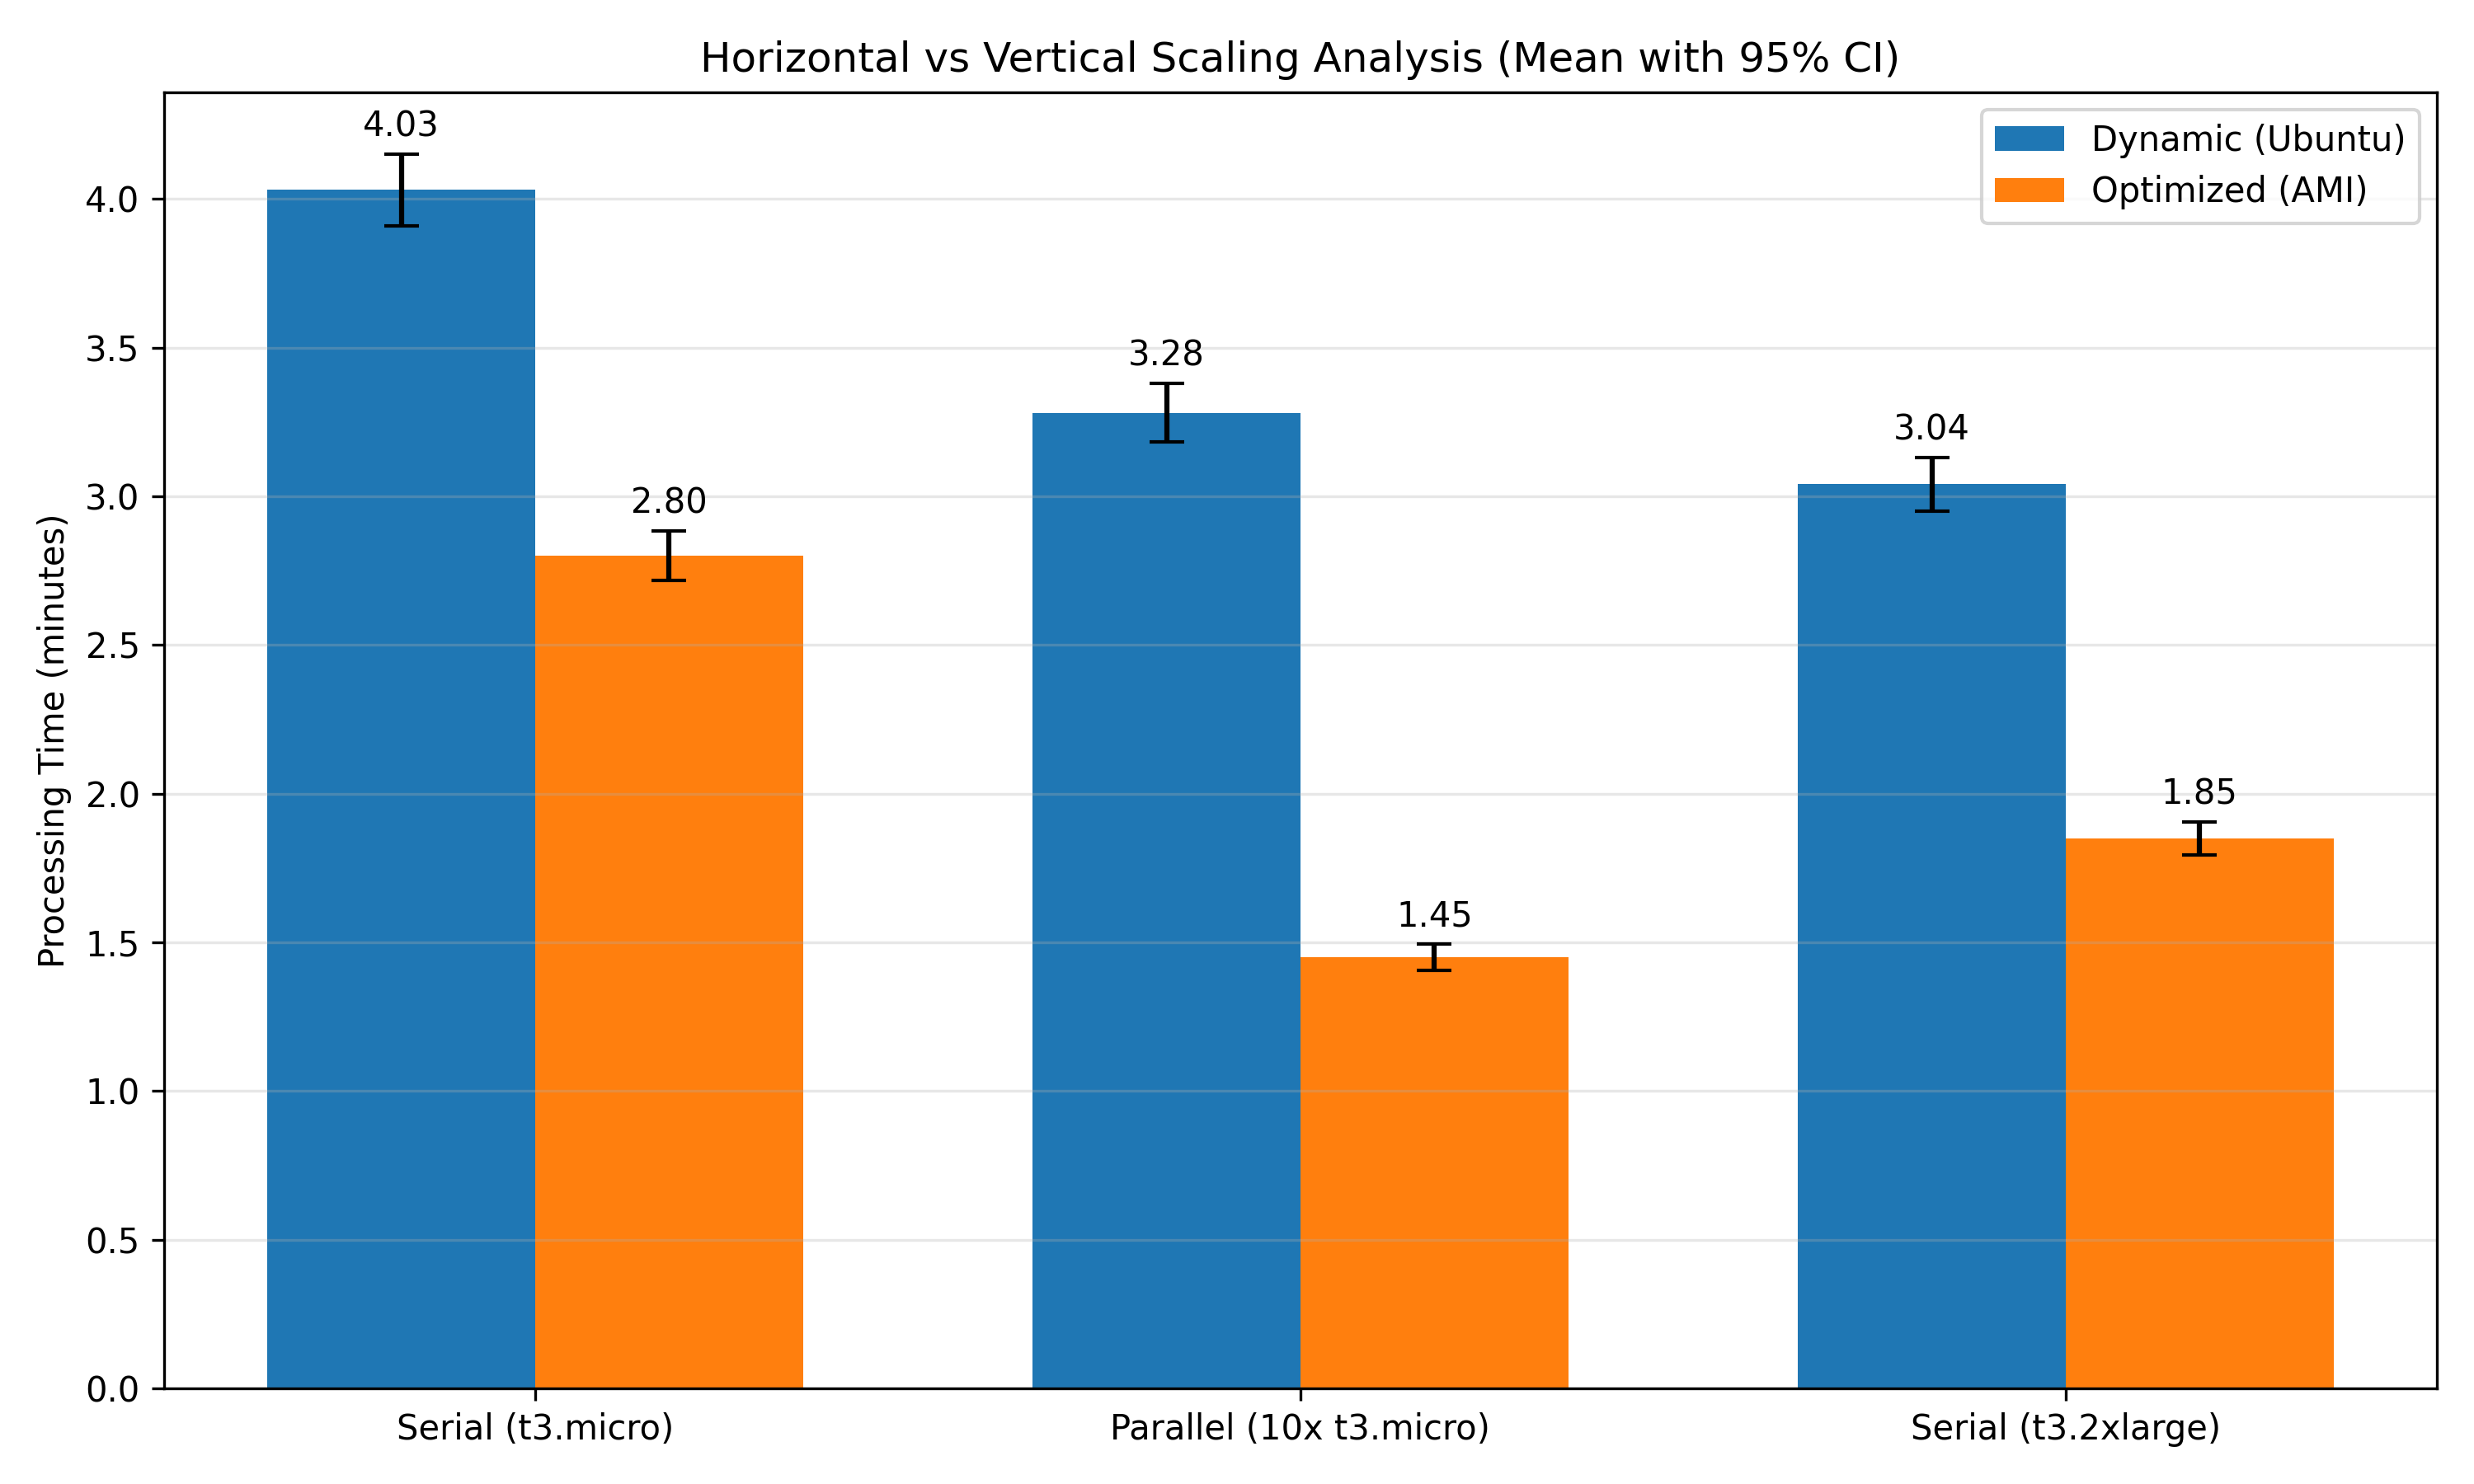
\includegraphics[width=0.5\textwidth]{graphs/comparison_time_cost_dual_axis.png}
		\caption{Performance and cost comparison between dynamic provisioning (Phase 3.1) and optimized provisioning (Phase 3.2). The dual-axis visualization demonstrates that horizontal scaling achieves superior performance and cost-efficiency when provisioning overhead is minimized through AMI optimization.}
		\label{fig:ami_comparison}
	\end{figure}
	
	\subsubsection{Methodological Validation of Scaling Conclusions}
	
	The experimental design provides robust validation for our conclusion that horizontal scaling outperforms vertical scaling for divisible video workloads, supported by the following methodological strengths:
	
	\begin{enumerate}
		\item \textbf{Controlled Comparison Methodology:} By testing identical workloads across both scaling strategies with identical optimization levels, we ensure fair comparison between architectural approaches. The 10-minute video segmentation for horizontal scaling versus integrated processing for vertical scaling represents equivalent computational workloads.
		
		\item \textbf{Bottleneck Quantification:} Provisioning overhead accounted for 70.2\% of total time in unoptimized deployments. A 57.4\% reduction in this overhead contributed to the observed performance improvements.
		
		\item \textbf{Statistical Significance and Reliability:} Multiple experimental runs (n=30 per configuration) provide statistical confidence in the observed performance differences. The consistent 1.28× performance improvement and 75.5\% cost reduction across optimization phases demonstrate reliable superiority of horizontal scaling.
		
		\item \textbf{Real-World Relevance and Practical Applicability:} The 10-minute video workload represents a practical use case, and the optimization strategy (custom AMIs) is directly applicable to production environments. The findings provide actionable guidance for cloud architecture decisions.
	\end{enumerate}
	
	The results demonstrate that horizontal scaling's theoretical advantages—parallel execution of independent workload segments—can be realized in practice when operational bottlenecks are addressed. The \textbf{75.5\% cost reduction} and \textbf{1.28× performance improvement} achieved through optimized horizontal scaling provide compelling evidence for re-evaluating conventional vertical scaling approaches for video encoding workloads.
	
	\subsubsection{Theoretical and Practical Implications}
	
	The Phase 3 results carry significant implications for both cloud computing theory and practice:
	
	\begin{itemize}
		\item \textbf{Theoretical Contribution:} Challenges established resource allocation paradigms that prioritize vertical scaling for performance-critical workloads, demonstrating that optimized horizontal scaling can simultaneously improve both performance and cost-efficiency.
		
		\item \textbf{Methodological Advancement:} Introduces a systematic approach for quantifying and mitigating provisioning overhead in cloud performance evaluations, addressing a frequently overlooked factor in scaling analyses.
		
		\item \textbf{Practical Architecture Guidance:} Provides empirical evidence supporting the use of cost-optimized instance clusters for divisible workloads, with specific optimization strategies (custom AMIs) that yield immediate practical benefits.
	\end{itemize}
	
	These findings establish that for divisible computational workloads like video encoding, horizontal scaling architectures utilizing cost-optimized instances represent the optimal strategy for maximizing both performance and economic efficiency in cloud environments.
	
	\section{Conclusion}
	\label{conclusion}
	
	This study demonstrates that architectural choices impact the cost-efficiency of video encoding in cloud environments. Our empirical analysis shows that smaller burstable instances (t3.micro) achieve up to 20× higher cost-effectiveness despite longer processing times, challenging conventional scaling assumptions. We quantified provisioning overhead, which consumed 70\% of total processing time in unoptimized parallel deployments. By eliminating this overhead through pre-configured machine images, we found that optimized horizontal scaling with t3.micro instances processes videos 1.28× faster while reducing costs by 75.5\% compared to vertical scaling.
	
	These findings have implications for cloud computing research and practice. The results challenge assumptions that raw computational power correlates with economic efficiency and establish provisioning overhead as a factor in distributed system performance. For practice, they indicate that pre-configured images are necessary for parallel encoding architectures, and that horizontal scaling with cost-optimized instances can outperform vertical scaling for divisible video workloads.
	
	Future research could extend this framework to additional media processing workloads, develop intelligent scaling systems that adapt instance counts based on real-time workload characterization, explore fault-tolerant patterns for spot instance utilization, and investigate performance variability in minimal instances. This research provides a foundation for efficient cloud resource utilization in media processing applications.
	\clearpage
	\begin{thebibliography}{00}
		\bibitem{b1} W. Maas, F. Rossi, M. Caggiani, P. Navaux, and A. Lorenzon, ``Investigating cloud instances to achieve optimal trade-offs between performance-cost efficiency,'' \emph{Computing}, vol. 107, no. 1, pp. 82--97, Jan. 2025. doi: 10.1007/s00607-025-01444-9.
		
		\bibitem{b2} P. Álvarez, S. Hernández, J. Fabra, and J. Ezpeleta, ``Cost-driven provisioning and execution of a computing-intensive service on the Amazon EC2,'' \emph{The Computer Journal}, vol. 61, no. 9, pp. 1407--1421, Jan. 2018. doi: 10.1093/comjnl/bxy006.
		
		\bibitem{b3} T. Dancheva, U. Alonso, and M. D. Barton, ``Cloud benchmarking and performance analysis of an HPC application in Amazon EC2,'' \emph{Cluster Computing}, vol. 27, no. 2, pp. 2273--2290, Jun. 2023. doi: 10.1007/s10586-023-04060-4.
		
		\bibitem{b4} L. M. Haji, S. R. M. Zeebaree, O. M. Ahmed, A. B. Sallow, K. Jacksi, and R. R. Zeabri, ``Dynamic Resource Allocation for Distributed Systems and Cloud Computing,'' \emph{Test Engineering and Management}, vol. 83, no. 1, pp. 22417--22426, Jun. 2020.
		
		\bibitem{b5} Z. Ou, H. Zhuang, J. K. Nurminen, A. Ylä-Jääski, and P. Hui, ``Exploiting Hardware Heterogeneity within the Same Instance Type of Amazon EC2,'' in \emph{Proc. 4th USENIX Conf. Hot Topics Cloud Comput.}, Boston, MA, USA, 2012, pp. 4--4.
		
		\bibitem{b6} Z. Ou, H. Zhuang, A. Lukyanenko, J. K. Nurminen, P. Hui, V. V. Mazalov, and A. Ylä-Jääski, ``Is the Same Instance Type Created Equal? Exploiting Heterogeneity of Public Clouds,'' \emph{IEEE Trans. Cloud Comput.}, vol. 1, no. 2, pp. 201--214, Jan. 2013. doi: 10.1109/TCC.2013.12.
		
		\bibitem{b7} B. Farley, A. Juels, V. Varadarajan, T. Ristenpart, K. D. Bowers, and M. M. Swift, ``More for Your Money: Exploiting Performance Heterogeneity in Public Clouds,'' in \emph{Proc. 3rd ACM Symp. Cloud Comput.}, San Jose, CA, USA, 2012, pp. 20:1--20:14. doi: 10.1145/2391229.2391249.
		
		\bibitem{b8} A. Katsenou, X. Wang, D. Schien, and D. Bull, ``Comparative Study of Hardware and Software Power Measurements in Video Compression,'' in \emph{2024 Picture Coding Symp. (PCS)}, Taichung, Taiwan, 2024, pp. 1--5. doi: 10.1109/PCS60826.2024.10566286.
		
		\bibitem{b9} A. Pereira Ferreira and R. O. Sinnott, ``A Performance Evaluation of Containers Running on Managed Kubernetes Services,'' in \emph{2019 IEEE Int. Conf. Cloud Comput. Technol. Sci. (CloudCom)}, Sydney, Australia, 2019, pp. 199--208. doi: 10.1109/CloudCom.2019.00038.
		
		\bibitem{b10} J. Scheuner and P. Leitner, ``Estimating Cloud Application Performance Based on Micro-Benchmark Profiling,'' in \emph{2018 IEEE 11th Int. Conf. Cloud Comput. (CLOUD)}, San Francisco, CA, USA, 2018, pp. 90--97. doi: 10.1109/CLOUD.2018.00019.
		
		\bibitem{b11} S. Ebneyousef and S. Ghazanfari-Rad, ``Cloud Resource Demand Prediction to Achieve Efficient Resource Provisioning,'' in \emph{2022 8th Iranian Conf. Signal Process. Intell. Syst. (ICSPIS)}, Tehran, Iran, 2022, pp. 1--6. doi: 10.1109/ICSPIS56952.2022.10043900.
		
		\bibitem{b12} T. S. Nikoui, A. Balador, A. M. Rahmani, and Z. Bakhshi, ``Cost-Aware Task Scheduling in Fog-Cloud Environment,'' in \emph{2020 CSI/CPSSI Int. Symp. Real-Time Embedded Syst. Technol. (RTEST)}, Tehran, Iran, 2020, pp. 1--8. doi: 10.1109/RTEST49666.2020.9140118.
		
		\bibitem{b13} Y. Yang and H. Casanova, ``RUMR: Robust Scheduling for Divisible Workloads,'' in \emph{Proc. 12th IEEE Int. Symp. High Perform. Distrib. Comput.}, Seattle, WA, USA, 2003, pp. 114--123. doi: 10.1109/HPDC.2003.1210021.
		
		\bibitem{b14} J. Praveenchandar and A. Tamilarasi, ``Resource Allocation Using Phase Change Hyper Switching Algorithm in the Cloud Environment,'' \emph{Intell. Autom. Soft Comput.}, vol. 34, no. 3, pp. 1839--1850, Aug. 2022. doi: 10.32604/iasc.2022.026354.
		
		\bibitem{b15} R. Rosado, O. Santos, F. Oliveira, L. Silva, G. Sanchez, I. Storch, D. Palomino, and L. Agostini, ``A Coding-Efficiency-Aware Fast Heuristic for VVC Intra-Frame Prediction Targeting 360° Videos,'' in \emph{Proc. 30th Brazilian Symp. Multimedia Web}, Juiz de Fora, Brazil, 2024, pp. 355--359. doi: 10.5753/webmedia.2024.243128.
		
		\bibitem{b16} L. Araújo, A. Duarte, G. Correa, B. Zatt, and D. Palomino, ``Fast ISP Mode Decision for the Versatile Video Coding Intra Prediction Using Machine Learning,'' in \emph{Proc. 30th Brazilian Symp. Multimedia Web}, Juiz de Fora, Brazil, 2024, pp. 162--170. doi: 10.5753/webmedia.2024.243129.
		
		\bibitem{b17} A. Mahida, ``Comprehensive Review on Optimizing Resource Allocation in Cloud Computing for Cost Efficiency,'' \emph{J. Artif. Intell. Cloud Comput.}, vol. 1, no. 2, pp. 1--4, May 2022. doi: 10.47363/JAICC/2022(1)232.
		
		\bibitem{b18} O. Alzakholi, L. M. Haji, H. M. Shukur, R. R. Zebari, S. M. Abas, and M. Sadeeq, ``Comparison Among Cloud Technologies and Cloud Performance,'' \emph{J. Appl. Sci. Technol. Trends}, vol. 1, no. 1, pp. 40--47, Apr. 2020. doi: 10.38094/jastt1219.
		
		\bibitem{b19} P. H. G. Silva, ``Analysis of SPOT Instance Pricing for Cost Minimization in a Multi-Cloud Context'' (In Portuguese), M.S. dissertation, Univ. Federal Pernambuco, Recife, Brazil, 2025.
		
		\bibitem{b20} F. Jiang, K. Ferriter, and C. Castillo, ``A Cloud-Agnostic Framework to Enable Cost-Aware Scheduling of Applications in a Multi-Cloud Environment,'' in \emph{2020 IEEE/IFIP Network Operations and Management Symposium (NOMS)}, Budapest, Hungary, 2020, pp. 1--9. doi: 10.1109/NOMS47738.2020.9110325.
		
	\end{thebibliography}
	
	\clearpage
	Appendix
	\section{Reproducibility and Data Availability}
	
	To ensure complete methodological transparency and enable independent verification of our findings, all experimental artifacts associated with this investigation have been made publicly accessible. This includes the complete instrumentation suite for instance provisioning, hardware verification, experimental orchestration, and data analysis, alongside comprehensive raw and aggregated datasets in standardized CSV format. These research artifacts are maintained in a public repository to facilitate scientific reproducibility and community validation.
	
	
\end{document}